
\let\negmedspace\undefined
\let\negthickspace\undefined
\documentclass[journal,12pt,twocolumn]{IEEEtran}
       \def\inputGnumericTable{}                                 %%
\usepackage{cite}
\usepackage{amsmath,amssymb,amsfonts,amsthm}
\usepackage{algorithmic}
\usepackage{graphicx}
\usepackage{textcomp}
\usepackage{xcolor}
\usepackage{txfonts}
\usepackage{listings}
\usepackage{enumitem}
\usepackage{mathtools}
\usepackage{gensymb}
\usepackage[breaklinks=true]{hyperref}
\usepackage{tkz-euclide} % loads  TikZ and tkz-base
\usepackage{listings}
\usepackage{gvv}
%
%\usepackage{setspace}
%\usepackage{gensymb}
%\doublespacing
%\singlespacing

%\usepackage{graphicx}
%\usepackage{amssymb}
%\usepackage{relsize}
%\usepackage[cmex10]{amsmath}
%\usepackage{amsthm}
%\interdisplaylinepenalty=2500
%\savesymbol{iint}
%\usepackage{txfonts}
%\restoresymbol{TXF}{iint}
%\usepackage{wasysym}
%\usepackage{amsthm}
%\usepackage{iithtlc}
%\usepackage{mathrsfs}
%\usepackage{txfonts}
%\usepackage{stfloats}
%\usepackage{bm}
%\usepackage{cite}
%\usepackage{cases}
%\usepackage{subfig}
%\usepackage{xtab}
%\usepackage{longtable}
%\usepackage{multirow}
%\usepackage{algorithm}
%\usepackage{algpseudocode}
%\usepackage{enumitem}
%\usepackage{mathtools}
%\usepackage{tikz}
%\usepackage{circuitikz}
%\usepackage{verbatim}
%\usepackage{tfrupee}
%\usepackage{stmaryrd}
%\usetkzobj{all}
    \usepackage{color}                                            %%
    \usepackage{array}                                            %%
    \usepackage{longtable}                                        %%
    \usepackage{calc}                                             %%
    \usepackage{multirow}                                         %%
    \usepackage{hhline}                                           %%
    \usepackage{ifthen}                                           %%
 %optionally (for landscape tables embedded in another document): %%
    \usepackage{lscape}     
%\usepackage{multicol}
%\usepackage{chngcntr}
%\usepackage{enumerate}

%\usepackage{wasysym}
%\documentclass[conference]{IEEEtran}
%\IEEEoverridecommandlockouts
% The preceding line is only needed to identify funding in the first footnote. If that is unneeded, please comment it out.

\newtheorem{theorem}{Theorem}[section]
\newtheorem{problem}{Problem}
\newtheorem{proposition}{Proposition}[section]
\newtheorem{lemma}{Lemma}[section]
\newtheorem{corollary}[theorem]{Corollary}
\newtheorem{example}{Example}[section]
\newtheorem{definition}[problem]{Definition}
%\newtheorem{thm}{Theorem}[section] 
%\newtheorem{defn}[thm]{Definition}
%\newtheorem{algorithm}{Algorithm}[section]
%\newtheorem{cor}{Corollary}
\newcommand{\BEQA}{\begin{eqnarray}}
\newcommand{\EEQA}{\end{eqnarray}}
\newcommand{\define}{\stackrel{\triangle}{=}}
\theoremstyle{remark}
\newtheorem{rem}{Remark}

%\bibliographystyle{ieeetr}
\begin{document}
Consider a triangle with vertices
\begin{align}
\vec {A} = \myvec {-4\\-3\\}\\
\vec {B} = \myvec {-6\\1\\}\\
\vec {C} = \myvec {-5\\-5\\}
\end{align}
\begin{table}[!ht]
        \centering
        \caption{Trianle}
	\label{table 1}	
	%%%%%%%%%%%%%%%%%%%%%%%%%%%%%%%%%%%%%%%%%%%%%%%%%%%%%%%%%%%%%%%%%%%%%%
%%                                                                  %%
%%  This is the header of a LaTeX2e file exported from Gnumeric.    %%
%%                                                                  %%
%%  This file can be compiled as it stands or included in another   %%
%%  LaTeX document. The table is based on the longtable package so  %%
%%  the longtable options (headers, footers...) can be set in the   %%
%%  preamble section below (see PRAMBLE).                           %%
%%                                                                  %%
%%  To include the file in another, the following two lines must be %%
%%  in the including file:                                          %%
%%        \def\inputGnumericTable{}                                 %%
%%  at the beginning of the file and:                               %%
%%        \input{name-of-this-file.tex}                             %%
%%  where the table is to be placed. Note also that the including   %%
%%  file must use the following packages for the table to be        %%
%%  rendered correctly:                                             %%
%%    \usepackage[latin1]{inputenc}                                 %%
%%    \usepackage{color}                                            %%
%%    \usepackage{array}                                            %%
%%    \usepackage{longtable}                                        %%
%%    \usepackage{calc}                                             %%
%%    \usepackage{multirow}                                         %%
%%    \usepackage{hhline}                                           %%
%%    \usepackage{ifthen}                                           %%
%%  optionally (for landscape tables embedded in another document): %%
%%    \usepackage{lscape}                                           %%
%%                                                                  %%
%%%%%%%%%%%%%%%%%%%%%%%%%%%%%%%%%%%%%%%%%%%%%%%%%%%%%%%%%%%%%%%%%%%%%%



%%  This section checks if we are begin input into another file or  %%
%%  the file will be compiled alone. First use a macro taken from   %%
%%  the TeXbook ex 7.7 (suggestion of Han-Wen Nienhuys).            %%
\def\ifundefined#1{\expandafter\ifx\csname#1\endcsname\relax}


%%  Check for the \def token for inputed files. If it is not        %%
%%  defined, the file will be processed as a standalone and the     %%
%%  preamble will be used.                                          %%
\ifundefined{inputGnumericTable}

%%  We must be able to close or not the document at the end.        %%
	\def\gnumericTableEnd{\end{document}}


%%%%%%%%%%%%%%%%%%%%%%%%%%%%%%%%%%%%%%%%%%%%%%%%%%%%%%%%%%%%%%%%%%%%%%
%%                                                                  %%
%%  This is the PREAMBLE. Change these values to get the right      %%
%%  paper size and other niceties.                                  %%
%%                                                                  %%
%%%%%%%%%%%%%%%%%%%%%%%%%%%%%%%%%%%%%%%%%%%%%%%%%%%%%%%%%%%%%%%%%%%%%%

	\documentclass[12pt%
			  %,landscape%
                    ]{report}
       \usepackage[latin1]{inputenc}
       \usepackage{fullpage}
       \usepackage{color}
       \usepackage{array}
       \usepackage{longtable}
       \usepackage{calc}
       \usepackage{multirow}
       \usepackage{hhline}
       \usepackage{ifthen}

	\begin{document}


%%  End of the preamble for the standalone. The next section is for %%
%%  documents which are included into other LaTeX2e files.          %%
\else

%%  We are not a stand alone document. For a regular table, we will %%
%%  have no preamble and only define the closing to mean nothing.   %%
    \def\gnumericTableEnd{}

%%  If we want landscape mode in an embedded document, comment out  %%
%%  the line above and uncomment the two below. The table will      %%
%%  begin on a new page and run in landscape mode.                  %%
%       \def\gnumericTableEnd{\end{landscape}}
%       \begin{landscape}


%%  End of the else clause for this file being \input.              %%
\fi

%%%%%%%%%%%%%%%%%%%%%%%%%%%%%%%%%%%%%%%%%%%%%%%%%%%%%%%%%%%%%%%%%%%%%%
%%                                                                  %%
%%  The rest is the gnumeric table, except for the closing          %%
%%  statement. Changes below will alter the table's appearance.     %%
%%                                                                  %%
%%%%%%%%%%%%%%%%%%%%%%%%%%%%%%%%%%%%%%%%%%%%%%%%%%%%%%%%%%%%%%%%%%%%%%

\providecommand{\gnumericmathit}[1]{#1} 
%%  Uncomment the next line if you would like your numbers to be in %%
%%  italics if they are italizised in the gnumeric table.           %%
%\renewcommand{\gnumericmathit}[1]{\mathit{#1}}
\providecommand{\gnumericPB}[1]%
{\let\gnumericTemp=\\#1\let\\=\gnumericTemp\hspace{0pt}}
 \ifundefined{gnumericTableWidthDefined}
        \newlength{\gnumericTableWidth}
        \newlength{\gnumericTableWidthComplete}
        \newlength{\gnumericMultiRowLength}
        \global\def\gnumericTableWidthDefined{}
 \fi
%% The following setting protects this code from babel shorthands.  %%
 \ifthenelse{\isundefined{\languageshorthands}}{}{\languageshorthands{english}}
%%  The default table format retains the relative column widths of  %%
%%  gnumeric. They can easily be changed to c, r or l. In that case %%
%%  you may want to comment out the next line and uncomment the one %%
%%  thereafter                                                      %%
\providecommand\gnumbox{\makebox[0pt]}
%%\providecommand\gnumbox[1][]{\makebox}

%% to adjust positions in multirow situations                       %%
\setlength{\bigstrutjot}{\jot}
\setlength{\extrarowheight}{\doublerulesep}

%%  The \setlongtables command keeps column widths the same across  %%
%%  pages. Simply comment out next line for varying column widths.  %%
\setlongtables

\setlength\gnumericTableWidth{%
	106pt+%
	106pt+%
	106pt+%
	106pt+%
	106pt+%
	106pt+%
	106pt+%
0pt}
\def\gumericNumCols{7}
\setlength\gnumericTableWidthComplete{\gnumericTableWidth+%
         \tabcolsep*\gumericNumCols*2+\arrayrulewidth*\gumericNumCols}
\ifthenelse{\lengthtest{\gnumericTableWidthComplete > \linewidth}}%
         {\def\gnumericScale{1*\ratio{\linewidth-%
                        \tabcolsep*\gumericNumCols*2-%
                        \arrayrulewidth*\gumericNumCols}%
{\gnumericTableWidth}}}%
{\def\gnumericScale{1}}

%%%%%%%%%%%%%%%%%%%%%%%%%%%%%%%%%%%%%%%%%%%%%%%%%%%%%%%%%%%%%%%%%%%%%%
%%                                                                  %%
%% The following are the widths of the various columns. We are      %%
%% defining them here because then they are easier to change.       %%
%% Depending on the cell formats we may use them more than once.    %%
%%                                                                  %%
%%%%%%%%%%%%%%%%%%%%%%%%%%%%%%%%%%%%%%%%%%%%%%%%%%%%%%%%%%%%%%%%%%%%%%

\ifthenelse{\isundefined{\gnumericColA}}{\newlength{\gnumericColA}}{}\settowidth{\gnumericColA}{\begin{tabular}{@{}p{106pt*\gnumericScale}@{}}x\end{tabular}}
\ifthenelse{\isundefined{\gnumericColB}}{\newlength{\gnumericColB}}{}\settowidth{\gnumericColB}{\begin{tabular}{@{}p{106pt*\gnumericScale}@{}}x\end{tabular}}
\ifthenelse{\isundefined{\gnumericColC}}{\newlength{\gnumericColC}}{}\settowidth{\gnumericColC}{\begin{tabular}{@{}p{106pt*\gnumericScale}@{}}x\end{tabular}}
\ifthenelse{\isundefined{\gnumericColD}}{\newlength{\gnumericColD}}{}\settowidth{\gnumericColD}{\begin{tabular}{@{}p{106pt*\gnumericScale}@{}}x\end{tabular}}
\ifthenelse{\isundefined{\gnumericColE}}{\newlength{\gnumericColE}}{}\settowidth{\gnumericColE}{\begin{tabular}{@{}p{106pt*\gnumericScale}@{}}x\end{tabular}}
\ifthenelse{\isundefined{\gnumericColF}}{\newlength{\gnumericColF}}{}\settowidth{\gnumericColF}{\begin{tabular}{@{}p{106pt*\gnumericScale}@{}}x\end{tabular}}
\ifthenelse{\isundefined{\gnumericColG}}{\newlength{\gnumericColG}}{}\settowidth{\gnumericColG}{\begin{tabular}{@{}p{106pt*\gnumericScale}@{}}x\end{tabular}}

\begin{tabular}[c]{%
	b{\gnumericColA}%
	b{\gnumericColB}%
	b{\gnumericColC}%
	b{\gnumericColD}%
	b{\gnumericColE}%
	b{\gnumericColF}%
	b{\gnumericColG}%
	}

%%%%%%%%%%%%%%%%%%%%%%%%%%%%%%%%%%%%%%%%%%%%%%%%%%%%%%%%%%%%%%%%%%%%%%
%%  The longtable options. (Caption, headers... see Goosens, p.124) %%
%	\caption{The Table Caption.}             \\	%
% \hline	% Across the top of the table.
%%  The rest of these options are table rows which are placed on    %%
%%  the first, last or every page. Use \multicolumn if you want.    %%

%%  Header for the first page.                                      %%
%	\multicolumn{7}{c}{The First Header} \\ \hline 
%	\multicolumn{1}{c}{colTag}	%Column 1
%	&\multicolumn{1}{c}{colTag}	%Column 2
%	&\multicolumn{1}{c}{colTag}	%Column 3
%	&\multicolumn{1}{c}{colTag}	%Column 4
%	&\multicolumn{1}{c}{colTag}	%Column 5
%	&\multicolumn{1}{c}{colTag}	%Column 6
%	&\multicolumn{1}{c}{colTag}	\\ \hline %Last column
%	\endfirsthead

%%  The running header definition.                                  %%
%	\hline
%	\multicolumn{7}{l}{\ldots\small\slshape continued} \\ \hline
%	\multicolumn{1}{c}{colTag}	%Column 1
%	&\multicolumn{1}{c}{colTag}	%Column 2
%	&\multicolumn{1}{c}{colTag}	%Column 3
%	&\multicolumn{1}{c}{colTag}	%Column 4
%	&\multicolumn{1}{c}{colTag}	%Column 5
%	&\multicolumn{1}{c}{colTag}	%Column 6
%	&\multicolumn{1}{c}{colTag}	\\ \hline %Last column
%	\endhead

%%  The running footer definition.                                  %%
%	\hline
%	\multicolumn{7}{r}{\small\slshape continued\ldots} \\
%	\endfoot

%%  The ending footer definition.                                   %%
%	\multicolumn{7}{c}{That's all folks} \\ \hline 
%	\endlastfoot
%%%%%%%%%%%%%%%%%%%%%%%%%%%%%%%%%%%%%%%%%%%%%%%%%%%%%%%%%%%%%%%%%%%%%%
\hhline{|--|--|---}
	 \multicolumn{2}{|p{	\gnumericColA+%
	\gnumericColB+%
	\tabcolsep*2*1}|}%
	{\gnumericPB{\centering}\gnumbox{parameters}}
	&\multicolumn{2}{p{	\gnumericColC+%
	\gnumericColD+%
	\tabcolsep*2*1}|}%
	{\gnumericPB{\centering}\gnumbox{values}}
	&\multicolumn{3}{p{	\gnumericColE+%
	\gnumericColF+%
	\gnumericColG+%
	\tabcolsep*2*2}|}%
	{\gnumericPB{\centering}\gnumbox{description}}
\\
\hhline{|-------|}
	 \multicolumn{2}{|p{	\gnumericColA+%
	\gnumericColB+%
	\tabcolsep*2*1}|}%
	{\gnumericPB{\centering}\gnumbox{$\vec{m_1}$}}
	&\multicolumn{2}{p{	\gnumericColC+%
	\gnumericColD+%
	\tabcolsep*2*1}|}%
	{\gnumericPB{\centering}\gnumbox{$\myvec{-2\\4\\}$}}
	&\multicolumn{3}{p{	\gnumericColE+%
	\gnumericColF+%
	\gnumericColG+%
	\tabcolsep*2*2}|}%
	{\gnumericPB{\centering}\gnumbox{$AB$}}
\\
\hhline{|-------|}
	 \multicolumn{2}{|p{	\gnumericColA+%
	\gnumericColB+%
	\tabcolsep*2*1}|}%
	{\gnumericPB{\centering}\gnumbox{$\vec{m_2}$}}
	&\multicolumn{2}{p{	\gnumericColC+%
	\gnumericColD+%
	\tabcolsep*2*1}|}%
	{\gnumericPB{\centering}\gnumbox{$\myvec{-1\\-6}$}}
	&\multicolumn{3}{p{	\gnumericColE+%
	\gnumericColF+%
	\gnumericColG+%
	\tabcolsep*2*2}|}%
	{\gnumericPB{\centering}\gnumbox{$BC$}}
\\
\hhline{|-------|}
	 \multicolumn{2}{|p{	\gnumericColA+%
	\gnumericColB+%
	\tabcolsep*2*1}|}%
	{\gnumericPB{\centering}\gnumbox{$\vec{m_3}$}}
	&\multicolumn{2}{p{	\gnumericColC+%
	\gnumericColD+%
	\tabcolsep*2*1}|}%
	{\gnumericPB{\centering}\gnumbox{$\myvec{1\\2}$}}
	&\multicolumn{3}{p{	\gnumericColE+%
	\gnumericColF+%
	\gnumericColG+%
	\tabcolsep*2*2}|}%
	{\gnumericPB{\centering}\gnumbox{$CA$}}
\\
\hhline{|-------|}
	 \multicolumn{2}{|p{	\gnumericColA+%
	\gnumericColB+%
	\tabcolsep*2*1}|}%
	{\gnumericPB{\centering}\gnumbox{$\norm{A-B}$}}
	&\multicolumn{2}{p{	\gnumericColC+%
	\gnumericColD+%
	\tabcolsep*2*1}|}%
	{\gnumericPB{\centering}\gnumbox{4.47}}
	&\multicolumn{3}{p{	\gnumericColE+%
	\gnumericColF+%
	\gnumericColG+%
	\tabcolsep*2*2}|}%
	{\gnumericPB{\centering}\gnumbox{length of $AB$}}
\\
\hhline{|-------|}
	 \multicolumn{2}{|p{	\gnumericColA+%
	\gnumericColB+%
	\tabcolsep*2*1}|}%
	{\gnumericPB{\centering}\gnumbox{$\norm{B-C}$}}
	&\multicolumn{2}{p{	\gnumericColC+%
	\gnumericColD+%
	\tabcolsep*2*1}|}%
	{\gnumericPB{\centering}\gnumbox{6.0827}}
	&\multicolumn{3}{p{	\gnumericColE+%
	\gnumericColF+%
	\gnumericColG+%
	\tabcolsep*2*2}|}%
	{\gnumericPB{\centering}\gnumbox{length of $BC$}}
\\
\hhline{|-------|}
	 \multicolumn{2}{|p{	\gnumericColA+%
	\gnumericColB+%
	\tabcolsep*2*1}|}%
	{\gnumericPB{\centering}\gnumbox{$\norm{C-A}$}}
	&\multicolumn{2}{p{	\gnumericColC+%
	\gnumericColD+%
	\tabcolsep*2*1}|}%
	{\gnumericPB{\centering}\gnumbox{2.236}}
	&\multicolumn{3}{p{	\gnumericColE+%
	\gnumericColF+%
	\gnumericColG+%
	\tabcolsep*2*2}|}%
	{\gnumericPB{\centering}\gnumbox{length of $CA$}}
\\
\hhline{|-------|}
	 \multicolumn{2}{|p{	\gnumericColA+%
	\gnumericColB+%
	\tabcolsep*3*1}|}%
	{\gnumericPB{\centering}\gnumbox{rank$\myvec{1&1&1\\\vec{A}&\vec{B}&\vec{C}}$}}
	&\multicolumn{2}{p{	\gnumericColC+%
	\gnumericColD+%
	\tabcolsep*2*1}|}%
	{\gnumericPB{\centering}\gnumbox{3}}
	&\multicolumn{3}{p{	\gnumericColE+%
	\gnumericColF+%
	\gnumericColG+%
	\tabcolsep*2*2}|}%
	{\gnumericPB{\centering}\gnumbox{non collinear}}
\\
\hhline{|-------|}
	 \multicolumn{2}{|p{	\gnumericColA+%
	\gnumericColB+%
	\tabcolsep*2*1}|}%
	{\gnumericPB{\centering}\gnumbox{$\vec{n_1}$}}
	&\multicolumn{2}{p{	\gnumericColC+%
	\gnumericColD+%
	\tabcolsep*2*1}|}%
	{\gnumericPB{\centering}\gnumbox{$\myvec{6\\1}$}}
	&\multicolumn{3}{c|}%
	{\setlength{\gnumericMultiRowLength}{0pt}%
	 \addtolength{\gnumericMultiRowLength}{\gnumericColE}%
	 \addtolength{\gnumericMultiRowLength}{\gnumericColF}%
	 \addtolength{\gnumericMultiRowLength}{\tabcolsep}%
	 \addtolength{\gnumericMultiRowLength}{\gnumericColG}%
	 \addtolength{\gnumericMultiRowLength}{\tabcolsep}%
	 \multirow{2}[1]{\gnumericMultiRowLength}{\parbox{\gnumericMultiRowLength}{%
	 \gnumericPB{\centering}\gnumbox{$AB$}}}}
\\
\hhline{|----|~~~}
	 \multicolumn{2}{|p{	\gnumericColA+%
	\gnumericColB+%
	\tabcolsep*2*1}|}%
	{\gnumericPB{\centering}\gnumbox{$c_1$}}
	&\multicolumn{2}{p{	\gnumericColC+%
	\gnumericColD+%
	\tabcolsep*2*1}|}%
	{\gnumericPB{\centering}\gnumbox{-35}}
	&
	&
	&\multicolumn{1}{p{\gnumericColG}|}%
	{}
\\
\hhline{|-------|}
	 \multicolumn{2}{|p{	\gnumericColA+%
	\gnumericColB+%
	\tabcolsep*2*1}|}%
	{\gnumericPB{\centering}\gnumbox{$\vec{n_2}$}}
	&\multicolumn{2}{p{	\gnumericColC+%
	\gnumericColD+%
	\tabcolsep*2*1}|}%
	{\gnumericPB{\centering}\gnumbox{$\myvec{-2\\1}$}}
	&\multicolumn{3}{c|}%
	{\setlength{\gnumericMultiRowLength}{0pt}%
	 \addtolength{\gnumericMultiRowLength}{\gnumericColE}%
	 \addtolength{\gnumericMultiRowLength}{\gnumericColF}%
	 \addtolength{\gnumericMultiRowLength}{\tabcolsep}%
	 \addtolength{\gnumericMultiRowLength}{\gnumericColG}%
	 \addtolength{\gnumericMultiRowLength}{\tabcolsep}%
	 \multirow{2}[1]{\gnumericMultiRowLength}{\parbox{\gnumericMultiRowLength}{%
	 \gnumericPB{\centering}\gnumbox{$BC$}}}}
\\
\hhline{|----|~~~}
	 \multicolumn{2}{|p{	\gnumericColA+%
	\gnumericColB+%
	\tabcolsep*2*1}|}%
	{\gnumericPB{\centering}\gnumbox{$c_2$}}
	&\multicolumn{2}{p{	\gnumericColC+%
	\gnumericColD+%
	\tabcolsep*2*1}|}%
	{\gnumericPB{\centering}\gnumbox{5}}
	&
	&
	&\multicolumn{1}{p{\gnumericColG}|}%
	{}
\\
\hhline{|-------|}
	 \multicolumn{2}{|p{	\gnumericColA+%
	\gnumericColB+%
	\tabcolsep*2*1}|}%
	{\gnumericPB{\centering}\gnumbox{$\vec{n_3}$}}
	&\multicolumn{2}{p{	\gnumericColC+%
	\gnumericColD+%
	\tabcolsep*2*1}|}%
	{\gnumericPB{\centering}\gnumbox{$\myvec{-4\\-2}$}}
	&\multicolumn{3}{c|}%
	{\setlength{\gnumericMultiRowLength}{0pt}%
	 \addtolength{\gnumericMultiRowLength}{\gnumericColE}%
	 \addtolength{\gnumericMultiRowLength}{\gnumericColF}%
	 \addtolength{\gnumericMultiRowLength}{\tabcolsep}%
	 \addtolength{\gnumericMultiRowLength}{\gnumericColG}%
	 \addtolength{\gnumericMultiRowLength}{\tabcolsep}%
	 \multirow{2}[1]{\gnumericMultiRowLength}{\parbox{\gnumericMultiRowLength}{%
	 \gnumericPB{\centering}\gnumbox{CA}}}}
\\
\hhline{|----|~~~}
	 \multicolumn{2}{|p{	\gnumericColA+%
	\gnumericColB+%
	\tabcolsep*2*1}|}%
	{\gnumericPB{\centering}\gnumbox{$c_3$}}
	&\multicolumn{2}{p{	\gnumericColC+%
	\gnumericColD+%
	\tabcolsep*2*1}|}%
	{\gnumericPB{\centering}\gnumbox{22}}
	&
	&
	&\multicolumn{1}{p{\gnumericColG}|}%
	{}
\\
\hhline{|-------|}
	 \multicolumn{2}{|p{	\gnumericColA+%
	\gnumericColB+%
	\tabcolsep*2*1}|}%
	{\gnumericPB{\centering}\gnumbox{Area}}
	&\multicolumn{2}{p{	\gnumericColC+%
	\gnumericColD+%
	\tabcolsep*2*1}|}%
	{\gnumericPB{\centering}\gnumbox{4}}
	&\multicolumn{3}{p{	\gnumericColE+%
	\gnumericColF+%
	\gnumericColG+%
	\tabcolsep*2*2}|}%
	{\gnumericPB{\centering}\gnumbox{Area of Triangle}}
\\
\hhline{|-------|}
	 \multicolumn{2}{|p{	\gnumericColA+%
	\gnumericColB+%
	\tabcolsep*2*1}|}%
	{\gnumericPB{\centering}\gnumbox{$\angle A$}}
	&\multicolumn{2}{p{	\gnumericColC+%
	\gnumericColD+%
	\tabcolsep*2*1}|}%
	{\gnumericPB{\centering}\gnumbox{$126.86\degree$}}
	&\multicolumn{3}{c|}%
	{\setlength{\gnumericMultiRowLength}{0pt}%
	 \addtolength{\gnumericMultiRowLength}{\gnumericColE}%
	 \addtolength{\gnumericMultiRowLength}{\gnumericColF}%
	 \addtolength{\gnumericMultiRowLength}{\tabcolsep}%
	 \addtolength{\gnumericMultiRowLength}{\gnumericColG}%
	 \addtolength{\gnumericMultiRowLength}{\tabcolsep}%
	 \multirow{3}[1]{\gnumericMultiRowLength}{\parbox{\gnumericMultiRowLength}{%
	 \gnumericPB{\centering}\gnumbox{Angles}}}}
\\
\hhline{|----|~~~}
	 \multicolumn{2}{|p{	\gnumericColA+%
	\gnumericColB+%
	\tabcolsep*2*1}|}%
	{\gnumericPB{\centering}\gnumbox{$\angle B$}}
	&\multicolumn{2}{p{	\gnumericColC+%
	\gnumericColD+%
	\tabcolsep*2*1}|}%
	{\gnumericPB{\centering}\gnumbox{$17.10\degree$}}
	&
	&
	&\multicolumn{1}{p{\gnumericColG}|}%
	{}
\\
\hhline{|----|~~~}
	 \multicolumn{2}{|p{	\gnumericColA+%
	\gnumericColB+%
	\tabcolsep*2*1}|}%
	{\gnumericPB{\centering}\gnumbox{$\angle C$}}
	&\multicolumn{2}{p{	\gnumericColC+%
	\gnumericColD+%
	\tabcolsep*2*1}|}%
	{\gnumericPB{\centering}\gnumbox{$36.02\degree$}}
	&
	&
	&\multicolumn{1}{p{\gnumericColG}|}%
	{}
\\
\hhline{|--|--|---|}
\end{tabular}

\ifthenelse{\isundefined{\languageshorthands}}{}{\languageshorthands{\languagename}}
\gnumericTableEnd

\end{table}
\begin{figure}[h!]
\centering
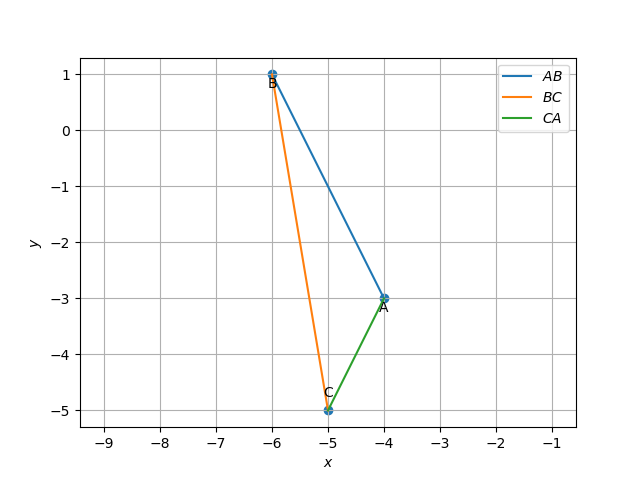
\includegraphics[width=0.8\linewidth] {/home/yogitha/triangle/figs/Fig1.png}
\caption{Sides}
\label{Fig1}
\end{figure}
\begin{table}[!ht]
        \centering
        \caption{Medians}
	\label{table 2}
	%%%%%%%%%%%%%%%%%%%%%%%%%%%%%%%%%%%%%%%%%%%%%%%%%%%%%%%%%%%%%%%%%%%%%%
%%                                                                  %%
%%  This is the header of a LaTeX2e file exported from Gnumeric.    %%
%%                                                                  %%
%%  This file can be compiled as it stands or included in another   %%
%%  LaTeX document. The table is based on the longtable package so  %%
%%  the longtable options (headers, footers...) can be set in the   %%
%%  preamble section below (see PRAMBLE).                           %%
%%                                                                  %%
%%  To include the file in another, the following two lines must be %%
%%  in the including file:                                          %%
%%        \def\inputGnumericTable{}                                 %%
%%  at the beginning of the file and:                               %%
%%        \input{name-of-this-file.tex}                             %%
%%  where the table is to be placed. Note also that the including   %%
%%  file must use the following packages for the table to be        %%
%%  rendered correctly:                                             %%
%%    \usepackage[latin1]{inputenc}                                 %%
%%    \usepackage{color}                                            %%
%%    \usepackage{array}                                            %%
%%    \usepackage{longtable}                                        %%
%%    \usepackage{calc}                                             %%
%%    \usepackage{multirow}                                         %%
%%    \usepackage{hhline}                                           %%
%%    \usepackage{ifthen}                                           %%
%%  optionally (for landscape tables embedded in another document): %%
%%    \usepackage{lscape}                                           %%
%%                                                                  %%
%%%%%%%%%%%%%%%%%%%%%%%%%%%%%%%%%%%%%%%%%%%%%%%%%%%%%%%%%%%%%%%%%%%%%%



%%  This section checks if we are begin input into another file or  %%
%%  the file will be compiled alone. First use a macro taken from   %%
%%  the TeXbook ex 7.7 (suggestion of Han-Wen Nienhuys).            %%
\def\ifundefined#1{\expandafter\ifx\csname#1\endcsname\relax}


%%  Check for the \def token for inputed files. If it is not        %%
%%  defined, the file will be processed as a standalone and the     %%
%%  preamble will be used.                                          %%
\ifundefined{inputGnumericTable}

%%  We must be able to close or not the document at the end.        %%
	\def\gnumericTableEnd{\end{document}}


%%%%%%%%%%%%%%%%%%%%%%%%%%%%%%%%%%%%%%%%%%%%%%%%%%%%%%%%%%%%%%%%%%%%%%
%%                                                                  %%
%%  This is the PREAMBLE. Change these values to get the right      %%
%%  paper size and other niceties.                                  %%
%%                                                                  %%
%%%%%%%%%%%%%%%%%%%%%%%%%%%%%%%%%%%%%%%%%%%%%%%%%%%%%%%%%%%%%%%%%%%%%%

	\documentclass[12pt%
			  %,landscape%
                    ]{report}
       \usepackage[latin1]{inputenc}
       \usepackage{fullpage}
       \usepackage{color}
       \usepackage{array}
       \usepackage{longtable}
       \usepackage{calc}
       \usepackage{multirow}
       \usepackage{hhline}
       \usepackage{ifthen}

	\begin{document}


%%  End of the preamble for the standalone. The next section is for %%
%%  documents which are included into other LaTeX2e files.          %%
\else

%%  We are not a stand alone document. For a regular table, we will %%
%%  have no preamble and only define the closing to mean nothing.   %%
    \def\gnumericTableEnd{}

%%  If we want landscape mode in an embedded document, comment out  %%
%%  the line above and uncomment the two below. The table will      %%
%%  begin on a new page and run in landscape mode.                  %%
%       \def\gnumericTableEnd{\end{landscape}}
%       \begin{landscape}


%%  End of the else clause for this file being \input.              %%
\fi

%%%%%%%%%%%%%%%%%%%%%%%%%%%%%%%%%%%%%%%%%%%%%%%%%%%%%%%%%%%%%%%%%%%%%%
%%                                                                  %%
%%  The rest is the gnumeric table, except for the closing          %%
%%  statement. Changes below will alter the table's appearance.     %%
%%                                                                  %%
%%%%%%%%%%%%%%%%%%%%%%%%%%%%%%%%%%%%%%%%%%%%%%%%%%%%%%%%%%%%%%%%%%%%%%

\providecommand{\gnumericmathit}[1]{#1} 
%%  Uncomment the next line if you would like your numbers to be in %%
%%  italics if they are italizised in the gnumeric table.           %%
%\renewcommand{\gnumericmathit}[1]{\mathit{#1}}
\providecommand{\gnumericPB}[1]%
{\let\gnumericTemp=\\#1\let\\=\gnumericTemp\hspace{0pt}}
 \ifundefined{gnumericTableWidthDefined}
        \newlength{\gnumericTableWidth}
        \newlength{\gnumericTableWidthComplete}
        \newlength{\gnumericMultiRowLength}
        \global\def\gnumericTableWidthDefined{}
 \fi
%% The following setting protects this code from babel shorthands.  %%
 \ifthenelse{\isundefined{\languageshorthands}}{}{\languageshorthands{english}}
%%  The default table format retains the relative column widths of  %%
%%  gnumeric. They can easily be changed to c, r or l. In that case %%
%%  you may want to comment out the next line and uncomment the one %%
%%  thereafter                                                      %%
\providecommand\gnumbox{\makebox[0pt]}
%%\providecommand\gnumbox[1][]{\makebox}

%% to adjust positions in multirow situations                       %%
\setlength{\bigstrutjot}{\jot}
\setlength{\extrarowheight}{\doublerulesep}

%%  The \setlongtables command keeps column widths the same across  %%
%%  pages. Simply comment out next line for varying column widths.  %%
\setlongtables

\setlength\gnumericTableWidth{%
	53pt+%
	53pt+%
	53pt+%
	53pt+%
	53pt+%
	53pt+%
	53pt+%
0pt}
\def\gumericNumCols{7}
\setlength\gnumericTableWidthComplete{\gnumericTableWidth+%
         \tabcolsep*\gumericNumCols*2+\arrayrulewidth*\gumericNumCols}
\ifthenelse{\lengthtest{\gnumericTableWidthComplete > \linewidth}}%
         {\def\gnumericScale{1*\ratio{\linewidth-%
                        \tabcolsep*\gumericNumCols*2-%
                        \arrayrulewidth*\gumericNumCols}%
{\gnumericTableWidth}}}%
{\def\gnumericScale{1}}

%%%%%%%%%%%%%%%%%%%%%%%%%%%%%%%%%%%%%%%%%%%%%%%%%%%%%%%%%%%%%%%%%%%%%%
%%                                                                  %%
%% The following are the widths of the various columns. We are      %%
%% defining them here because then they are easier to change.       %%
%% Depending on the cell formats we may use them more than once.    %%
%%                                                                  %%
%%%%%%%%%%%%%%%%%%%%%%%%%%%%%%%%%%%%%%%%%%%%%%%%%%%%%%%%%%%%%%%%%%%%%%

\ifthenelse{\isundefined{\gnumericColA}}{\newlength{\gnumericColA}}{}\settowidth{\gnumericColA}{\begin{tabular}{@{}p{53pt*\gnumericScale}@{}}x\end{tabular}}
\ifthenelse{\isundefined{\gnumericColB}}{\newlength{\gnumericColB}}{}\settowidth{\gnumericColB}{\begin{tabular}{@{}p{53pt*\gnumericScale}@{}}x\end{tabular}}
\ifthenelse{\isundefined{\gnumericColC}}{\newlength{\gnumericColC}}{}\settowidth{\gnumericColC}{\begin{tabular}{@{}p{53pt*\gnumericScale}@{}}x\end{tabular}}
\ifthenelse{\isundefined{\gnumericColD}}{\newlength{\gnumericColD}}{}\settowidth{\gnumericColD}{\begin{tabular}{@{}p{53pt*\gnumericScale}@{}}x\end{tabular}}
\ifthenelse{\isundefined{\gnumericColE}}{\newlength{\gnumericColE}}{}\settowidth{\gnumericColE}{\begin{tabular}{@{}p{53pt*\gnumericScale}@{}}x\end{tabular}}
\ifthenelse{\isundefined{\gnumericColF}}{\newlength{\gnumericColF}}{}\settowidth{\gnumericColF}{\begin{tabular}{@{}p{53pt*\gnumericScale}@{}}x\end{tabular}}
\ifthenelse{\isundefined{\gnumericColG}}{\newlength{\gnumericColG}}{}\settowidth{\gnumericColG}{\begin{tabular}{@{}p{53pt*\gnumericScale}@{}}x\end{tabular}}

\begin{tabular}[c]{%
	b{\gnumericColA}%
	b{\gnumericColB}%
	b{\gnumericColC}%
	b{\gnumericColD}%
	b{\gnumericColE}%
	b{\gnumericColF}%
	b{\gnumericColG}%
	}

%%%%%%%%%%%%%%%%%%%%%%%%%%%%%%%%%%%%%%%%%%%%%%%%%%%%%%%%%%%%%%%%%%%%%%
%%  The longtable options. (Caption, headers... see Goosens, p.124) %%
%	\caption{The Table Caption.}             \\	%
% \hline	% Across the top of the table.
%%  The rest of these options are table rows which are placed on    %%
%%  the first, last or every page. Use \multicolumn if you want.    %%

%%  Header for the first page.                                      %%
%	\multicolumn{7}{c}{The First Header} \\ \hline 
%	\multicolumn{1}{c}{colTag}	%Column 1
%	&\multicolumn{1}{c}{colTag}	%Column 2
%	&\multicolumn{1}{c}{colTag}	%Column 3
%	&\multicolumn{1}{c}{colTag}	%Column 4
%	&\multicolumn{1}{c}{colTag}	%Column 5
%	&\multicolumn{1}{c}{colTag}	%Column 6
%	&\multicolumn{1}{c}{colTag}	\\ \hline %Last column
%	\endfirsthead

%%  The running header definition.                                  %%
%	\hline
%	\multicolumn{7}{l}{\ldots\small\slshape continued} \\ \hline
%	\multicolumn{1}{c}{colTag}	%Column 1
%	&\multicolumn{1}{c}{colTag}	%Column 2
%	&\multicolumn{1}{c}{colTag}	%Column 3
%	&\multicolumn{1}{c}{colTag}	%Column 4
%	&\multicolumn{1}{c}{colTag}	%Column 5
%	&\multicolumn{1}{c}{colTag}	%Column 6
%	&\multicolumn{1}{c}{colTag}	\\ \hline %Last column
%	\endhead

%%  The running footer definition.                                  %%
%	\hline
%	\multicolumn{7}{r}{\small\slshape continued\ldots} \\
%	\endfoot

%%  The ending footer definition.                                   %%
%	\multicolumn{7}{c}{That's all folks} \\ \hline 
%	\endlastfoot
%%%%%%%%%%%%%%%%%%%%%%%%%%%%%%%%%%%%%%%%%%%%%%%%%%%%%%%%%%%%%%%%%%%%%%

\hhline{|--|--|---}
	 \multicolumn{2}{|p{	\gnumericColA+%
	\gnumericColB+%
	\tabcolsep*2*1}|}%
	{\gnumericPB{\centering}\gnumbox{parameters}}
	&\multicolumn{2}{p{	\gnumericColC+%
	\gnumericColD+%
	\tabcolsep*2*1}|}%
	{\gnumericPB{\centering}\gnumbox{value}}
	&\multicolumn{3}{p{	\gnumericColE+%
	\gnumericColF+%
	\gnumericColG+%
	\tabcolsep*2*2}|}%
	{\gnumericPB{\centering}\gnumbox{description}}
\\
\hhline{|-------|}
	 \multicolumn{2}{|p{	\gnumericColA+%
	\gnumericColB+%
	\tabcolsep*2*1}|}%
	{\gnumericPB{\centering}\gnumbox{$\vec{D}$}}
	&\multicolumn{2}{p{	\gnumericColC+%
	\gnumericColD+%
	\tabcolsep*2*1}|}%
	{\gnumericPB{\centering}\gnumbox{$\myvec{3\\2}$}}
	&\multicolumn{3}{p{	\gnumericColE+%
	\gnumericColF+%
	\gnumericColG+%
	\tabcolsep*2*2}|}%
	{\gnumericPB{\centering}\gnumbox{$BC$ midpoint}}
\\
\hhline{|-------|}
	 \multicolumn{2}{|p{	\gnumericColA+%
	\gnumericColB+%
	\tabcolsep*2*1}|}%
	{\gnumericPB{\centering}\gnumbox{$\vec{E}$}}
	&\multicolumn{2}{p{	\gnumericColC+%
	\gnumericColD+%
	\tabcolsep*2*1}|}%
	{\gnumericPB{\centering}\gnumbox{$\myvec{2\\0}$}}
	&\multicolumn{3}{p{	\gnumericColE+%
	\gnumericColF+%
	\gnumericColG+%
	\tabcolsep*2*2}|}%
	{\gnumericPB{\centering}\gnumbox{$CA$ midpoint}}
\\
\hhline{|-------|}
	 \multicolumn{2}{|p{	\gnumericColA+%
	\gnumericColB+%
	\tabcolsep*2*1}|}%
	{\gnumericPB{\centering}\gnumbox{$\vec{F}$}}
	&\multicolumn{2}{p{	\gnumericColC+%
	\gnumericColD+%
	\tabcolsep*2*1}|}%
	{\gnumericPB{\centering}\gnumbox{$\myvec{3\\1}$}}
	&\multicolumn{3}{p{	\gnumericColE+%
	\gnumericColF+%
	\gnumericColG+%
	\tabcolsep*2*2}|}%
	{\gnumericPB{\centering}\gnumbox{$AB$ midpoint}}
\\
\hhline{|-------|}
	 \multicolumn{2}{|p{	\gnumericColA+%
	\gnumericColB+%
	\tabcolsep*2*1}|}%
	{\gnumericPB{\centering}\gnumbox{$\vec{m_4}$}}
	&\multicolumn{2}{p{	\gnumericColC+%
	\gnumericColD+%
	\tabcolsep*2*1}|}%
	{\gnumericPB{\centering}\gnumbox{$\myvec{1\\3}$}}
	&\multicolumn{3}{c|}%
	{\setlength{\gnumericMultiRowLength}{0pt}%
	 \addtolength{\gnumericMultiRowLength}{\gnumericColE}%
	 \addtolength{\gnumericMultiRowLength}{\gnumericColF}%
	 \addtolength{\gnumericMultiRowLength}{\tabcolsep}%
	 \addtolength{\gnumericMultiRowLength}{\gnumericColG}%
	 \addtolength{\gnumericMultiRowLength}{\tabcolsep}%
	 \multirow{3}[1]{\gnumericMultiRowLength}{\parbox{\gnumericMultiRowLength}{%
	 \gnumericPB{\centering}\gnumbox{$AD$}}}}
\\
\hhline{|----|~~~}
	 \multicolumn{2}{|p{	\gnumericColA+%
	\gnumericColB+%
	\tabcolsep*2*1}|}%
	{\gnumericPB{\centering}\gnumbox{$\vec{n_4}$}}
	&\multicolumn{2}{p{	\gnumericColC+%
	\gnumericColD+%
	\tabcolsep*2*1}|}%
	{\gnumericPB{\centering}\gnumbox{$\myvec{3\\-1}$}}
	&
	&
	&\multicolumn{1}{p{\gnumericColG}|}%
	{}
\\
\hhline{|----|~~~}
	 \multicolumn{2}{|p{	\gnumericColA+%
	\gnumericColB+%
	\tabcolsep*2*1}|}%
	{\gnumericPB{\centering}\gnumbox{$c_4$}}
	&\multicolumn{2}{p{	\gnumericColC+%
	\gnumericColD+%
	\tabcolsep*2*1}|}%
	{\gnumericPB{\centering}\gnumbox{7}}
	&
	&
	&\multicolumn{1}{p{\gnumericColG}|}%
	{}
\\
\hhline{|-------|}
	 \multicolumn{2}{|p{	\gnumericColA+%
	\gnumericColB+%
	\tabcolsep*2*1}|}%
	{\gnumericPB{\centering}\gnumbox{$\vec{m_5}$}}
	&\multicolumn{2}{p{	\gnumericColC+%
	\gnumericColD+%
	\tabcolsep*2*1}|}%
	{\gnumericPB{\centering}\gnumbox{$\myvec{-2\\-3}$}}
	&\multicolumn{3}{c|}%
	{\setlength{\gnumericMultiRowLength}{0pt}%
	 \addtolength{\gnumericMultiRowLength}{\gnumericColE}%
	 \addtolength{\gnumericMultiRowLength}{\gnumericColF}%
	 \addtolength{\gnumericMultiRowLength}{\tabcolsep}%
	 \addtolength{\gnumericMultiRowLength}{\gnumericColG}%
	 \addtolength{\gnumericMultiRowLength}{\tabcolsep}%
	 \multirow{3}[1]{\gnumericMultiRowLength}{\parbox{\gnumericMultiRowLength}{%
	 \gnumericPB{\centering}\gnumbox{$BE$}}}}
\\
\hhline{|----|~~~}
	 \multicolumn{2}{|p{	\gnumericColA+%
	\gnumericColB+%
	\tabcolsep*2*1}|}%
	{\gnumericPB{\centering}\gnumbox{$\vec{n_5}$}}
	&\multicolumn{2}{p{	\gnumericColC+%
	\gnumericColD+%
	\tabcolsep*2*1}|}%
	{\gnumericPB{\centering}\gnumbox{$\myvec{-3\\2}$}}
	&
	&
	&\multicolumn{1}{p{\gnumericColG}|}%
	{}
\\
\hhline{|----|~~~}
	 \multicolumn{2}{|p{	\gnumericColA+%
	\gnumericColB+%
	\tabcolsep*2*1}|}%
	{\gnumericPB{\centering}\gnumbox{$c_5$}}
	&\multicolumn{2}{p{	\gnumericColC+%
	\gnumericColD+%
	\tabcolsep*2*1}|}%
	{\gnumericPB{\centering}\gnumbox{-6}}
	&
	&
	&\multicolumn{1}{p{\gnumericColG}|}%
	{}
\\
\hhline{|-------|}
	 \multicolumn{2}{|p{	\gnumericColA+%
	\gnumericColB+%
	\tabcolsep*2*1}|}%
	{\gnumericPB{\centering}\gnumbox{$\vec{m_6}$}}
	&\multicolumn{2}{p{	\gnumericColC+%
	\gnumericColD+%
	\tabcolsep*2*1}|}%
	{\gnumericPB{\centering}\gnumbox{$\myvec{1\\0}$}}
	&\multicolumn{3}{c|}%
	{\setlength{\gnumericMultiRowLength}{0pt}%
	 \addtolength{\gnumericMultiRowLength}{\gnumericColE}%
	 \addtolength{\gnumericMultiRowLength}{\gnumericColF}%
	 \addtolength{\gnumericMultiRowLength}{\tabcolsep}%
	 \addtolength{\gnumericMultiRowLength}{\gnumericColG}%
	 \addtolength{\gnumericMultiRowLength}{\tabcolsep}%
	 \multirow{3}[1]{\gnumericMultiRowLength}{\parbox{\gnumericMultiRowLength}{%
	 \gnumericPB{\centering}\gnumbox{$CF$}}}}
\\
\hhline{|----|~~~}
	 \multicolumn{2}{|p{	\gnumericColA+%
	\gnumericColB+%
	\tabcolsep*2*1}|}%
	{\gnumericPB{\centering}\gnumbox{$\vec{n_6}$}}
	&\multicolumn{2}{p{	\gnumericColC+%
	\gnumericColD+%
	\tabcolsep*2*1}|}%
	{\gnumericPB{\centering}\gnumbox{$\myvec{0\\-1}$}}
	&
	&
	&\multicolumn{1}{p{\gnumericColG}|}%
	{}
\\
\hhline{|----|~~~}
	 \multicolumn{2}{|p{	\gnumericColA+%
	\gnumericColB+%
	\tabcolsep*2*1}|}%
	{\gnumericPB{\centering}\gnumbox{$c_6$}}
	&\multicolumn{2}{p{	\gnumericColC+%
	\gnumericColD+%
	\tabcolsep*2*1}|}%
	{\gnumericPB{\centering}\gnumbox{-1}}
	&
	&
	&\multicolumn{1}{p{\gnumericColG}|}%
	{}
\\
\hhline{|-------|}
	 \multicolumn{2}{|p{	\gnumericColA+%
	\gnumericColB+%
	\tabcolsep*2*1}|}%
	{\gnumericPB{\centering}\gnumbox{$\vec{G}$}}
	&\multicolumn{2}{p{	\gnumericColC+%
	\gnumericColD+%
	\tabcolsep*2*1}|}%
	{\gnumericPB{\centering}\gnumbox{$\myvec{2.67\\1}$}}
	&\multicolumn{3}{p{	\gnumericColE+%
	\gnumericColF+%
	\gnumericColG+%
	\tabcolsep*2*2}|}%
	{\gnumericPB{\centering}\gnumbox{Centroid}}
\\
\hhline{|-------|}
	 \multicolumn{2}{|p{	\gnumericColA+%
	\gnumericColB+%
	\tabcolsep*2*1}|}%
	{\gnumericPB{\centering}\gnumbox{$\frac{BG}{GE}$}}
	&\multicolumn{2}{c|}%
	{\setlength{\gnumericMultiRowLength}{0pt}%
	 \addtolength{\gnumericMultiRowLength}{\gnumericColC}%
	 \addtolength{\gnumericMultiRowLength}{\gnumericColD}%
	 \addtolength{\gnumericMultiRowLength}{\tabcolsep}%
	 \multirow{3}[1]{\gnumericMultiRowLength}{\parbox{\gnumericMultiRowLength}{%
	 \gnumericPB{\centering}\gnumbox{2}}}}
	&\multicolumn{3}{c|}%
	{\setlength{\gnumericMultiRowLength}{0pt}%
	 \addtolength{\gnumericMultiRowLength}{\gnumericColE}%
	 \addtolength{\gnumericMultiRowLength}{\gnumericColF}%
	 \addtolength{\gnumericMultiRowLength}{\tabcolsep}%
	 \addtolength{\gnumericMultiRowLength}{\gnumericColG}%
	 \addtolength{\gnumericMultiRowLength}{\tabcolsep}%
	 \multirow{3}[1]{\gnumericMultiRowLength}{\parbox{\gnumericMultiRowLength}{%
	 \gnumericPB{\centering}\gnumbox{Division ratio by $\vec{G}$}}}}
\\
\hhline{|--|~~~~~}
	 \multicolumn{2}{|p{	\gnumericColA+%
	\gnumericColB+%
	\tabcolsep*2*1}|}%
	{\gnumericPB{\centering}\gnumbox{$\frac{CG}{GF}$}}
	&
	&\multicolumn{1}{p{\gnumericColD}|}%
	{}
	&
	&
	&\multicolumn{1}{p{\gnumericColG}|}%
	{}
\\
\hhline{|--|~~~~~}
	 \multicolumn{2}{|p{	\gnumericColA+%
	\gnumericColB+%
	\tabcolsep*2*1}|}%
	{\gnumericPB{\centering}\gnumbox{$\frac{AG}{GD}$}}
	&
	&\multicolumn{1}{p{\gnumericColD}|}%
	{}
	&
	&
	&\multicolumn{1}{p{\gnumericColG}|}%
	{}
\\
\hhline{|-------|}
	 \multicolumn{2}{|p{	\gnumericColA+%
	\gnumericColB+%
	\tabcolsep*2*1}|}%
	{\gnumericPB{\centering}\gnumbox{rank$\myvec{1&1&1\\\vec{A}&\vec{D}&\vec{G}}$}}
	&\multicolumn{2}{c|}%
	{\setlength{\gnumericMultiRowLength}{0pt}%
	 \addtolength{\gnumericMultiRowLength}{\gnumericColC}%
	 \addtolength{\gnumericMultiRowLength}{\gnumericColD}%
	 \addtolength{\gnumericMultiRowLength}{\tabcolsep}%
	 \multirow{3}[1]{\gnumericMultiRowLength}{\parbox{\gnumericMultiRowLength}{%
	 \gnumericPB{\centering}\gnumbox{2}}}}
	&\multicolumn{3}{c|}%
	{\setlength{\gnumericMultiRowLength}{0pt}%
	 \addtolength{\gnumericMultiRowLength}{\gnumericColE}%
	 \addtolength{\gnumericMultiRowLength}{\gnumericColF}%
	 \addtolength{\gnumericMultiRowLength}{\tabcolsep}%
	 \addtolength{\gnumericMultiRowLength}{\gnumericColG}%
	 \addtolength{\gnumericMultiRowLength}{\tabcolsep}%
	 \multirow{3}[1]{\gnumericMultiRowLength}{\parbox{\gnumericMultiRowLength}{%
	 \gnumericPB{\centering}\gnumbox{collinear}}}}
\\
\hhline{|--|~~~~~}
	 \multicolumn{2}{|p{	\gnumericColA+%
	\gnumericColB+%
	\tabcolsep*2*1}|}%
	{\gnumericPB{\centering}\gnumbox{rank$\myvec{1&1&1\\\vec{B}&\vec{E}&\vec{G}}$}}
	&
	&\multicolumn{1}{p{\gnumericColD}|}%
	{}
	&
	&
	&\multicolumn{1}{p{\gnumericColG}|}%
	{}
\\
\hhline{|--|~~~~~}
	 \multicolumn{2}{|p{	\gnumericColA+%
	\gnumericColB+%
	\tabcolsep*2*1}|}%
	{\gnumericPB{\centering}\gnumbox{rank$\myvec{1&1&1\\\vec{C}&\vec{F}&\vec{G}}$}}
	&
	&\multicolumn{1}{p{\gnumericColD}|}%
	{}
	&
	&
	&\multicolumn{1}{p{\gnumericColG}|}%
	{}
\\
\hhline{|--|--|---|}
\end{tabular}

\ifthenelse{\isundefined{\languageshorthands}}{}{\languageshorthands{\languagename}}
\gnumericTableEnd

\end{table}
\begin{figure}[h!]
\centering
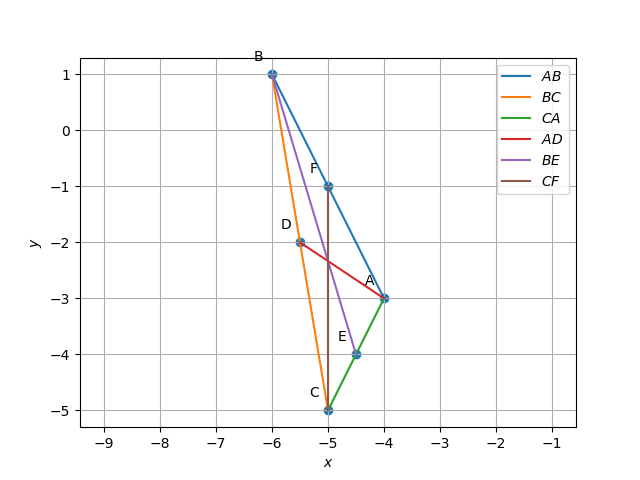
\includegraphics[width=0.8\linewidth] {/home/yogitha/triangle/figs/Fig2.png}
\caption{Medians}
\label{fig2}
\end{figure}
\begin{table}[!ht]
        \centering
	\caption{Medians}
	\label{table 3}
	%%%%%%%%%%%%%%%%%%%%%%%%%%%%%%%%%%%%%%%%%%%%%%%%%%%%%%%%%%%%%%%%%%%%%%
%%                                                                  %%
%%  This is the header of a LaTeX2e file exported from Gnumeric.    %%
%%                                                                  %%
%%  This file can be compiled as it stands or included in another   %%
%%  LaTeX document. The table is based on the longtable package so  %%
%%  the longtable options (headers, footers...) can be set in the   %%
%%  preamble section below (see PRAMBLE).                           %%
%%                                                                  %%
%%  To include the file in another, the following two lines must be %%
%%  in the including file:                                          %%
%%        \def\inputGnumericTable{}                                 %%
%%  at the beginning of the file and:                               %%
%%        \input{name-of-this-file.tex}                             %%
%%  where the table is to be placed. Note also that the including   %%
%%  file must use the following packages for the table to be        %%
%%  rendered correctly:                                             %%
%%    \usepackage[latin1]{inputenc}                                 %%
%%    \usepackage{color}                                            %%
%%    \usepackage{array}                                            %%
%%    \usepackage{longtable}                                        %%
%%    \usepackage{calc}                                             %%
%%    \usepackage{multirow}                                         %%
%%    \usepackage{hhline}                                           %%
%%    \usepackage{ifthen}                                           %%
%%  optionally (for landscape tables embedded in another document): %%
%%    \usepackage{lscape}                                           %%
%%                                                                  %%
%%%%%%%%%%%%%%%%%%%%%%%%%%%%%%%%%%%%%%%%%%%%%%%%%%%%%%%%%%%%%%%%%%%%%%



%%  This section checks if we are begin input into another file or  %%
%%  the file will be compiled alone. First use a macro taken from   %%
%%  the TeXbook ex 7.7 (suggestion of Han-Wen Nienhuys).            %%
\def\ifundefined#1{\expandafter\ifx\csname#1\endcsname\relax}


%%  Check for the \def token for inputed files. If it is not        %%
%%  defined, the file will be processed as a standalone and the     %%
%%  preamble will be used.                                          %%
\ifundefined{inputGnumericTable}

%%  We must be able to close or not the document at the end.        %%
	\def\gnumericTableEnd{\end{document}}


%%%%%%%%%%%%%%%%%%%%%%%%%%%%%%%%%%%%%%%%%%%%%%%%%%%%%%%%%%%%%%%%%%%%%%
%%                                                                  %%
%%  This is the PREAMBLE. Change these values to get the right      %%
%%  paper size and other niceties.                                  %%
%%                                                                  %%
%%%%%%%%%%%%%%%%%%%%%%%%%%%%%%%%%%%%%%%%%%%%%%%%%%%%%%%%%%%%%%%%%%%%%%

	\documentclass[12pt%
			  %,landscape%
                    ]{report}
       \usepackage[latin1]{inputenc}
       \usepackage{fullpage}
       \usepackage{color}
       \usepackage{array}
       \usepackage{longtable}
       \usepackage{calc}
       \usepackage{multirow}
       \usepackage{hhline}
       \usepackage{ifthen}

	\begin{document}


%%  End of the preamble for the standalone. The next section is for %%
%%  documents which are included into other LaTeX2e files.          %%
\else

%%  We are not a stand alone document. For a regular table, we will %%
%%  have no preamble and only define the closing to mean nothing.   %%
    \def\gnumericTableEnd{}

%%  If we want landscape mode in an embedded document, comment out  %%
%%  the line above and uncomment the two below. The table will      %%
%%  begin on a new page and run in landscape mode.                  %%
%       \def\gnumericTableEnd{\end{landscape}}
%       \begin{landscape}


%%  End of the else clause for this file being \input.              %%
\fi

%%%%%%%%%%%%%%%%%%%%%%%%%%%%%%%%%%%%%%%%%%%%%%%%%%%%%%%%%%%%%%%%%%%%%%
%%                                                                  %%
%%  The rest is the gnumeric table, except for the closing          %%
%%  statement. Changes below will alter the table's appearance.     %%
%%                                                                  %%
%%%%%%%%%%%%%%%%%%%%%%%%%%%%%%%%%%%%%%%%%%%%%%%%%%%%%%%%%%%%%%%%%%%%%%

\providecommand{\gnumericmathit}[1]{#1} 
%%  Uncomment the next line if you would like your numbers to be in %%
%%  italics if they are italizised in the gnumeric table.           %%
%\renewcommand{\gnumericmathit}[1]{\mathit{#1}}
\providecommand{\gnumericPB}[1]%
{\let\gnumericTemp=\\#1\let\\=\gnumericTemp\hspace{0pt}}
 \ifundefined{gnumericTableWidthDefined}
        \newlength{\gnumericTableWidth}
        \newlength{\gnumericTableWidthComplete}
        \newlength{\gnumericMultiRowLength}
        \global\def\gnumericTableWidthDefined{}
 \fi
%% The following setting protects this code from babel shorthands.  %%
 \ifthenelse{\isundefined{\languageshorthands}}{}{\languageshorthands{english}}
%%  The default table format retains the relative column widths of  %%
%%  gnumeric. They can easily be changed to c, r or l. In that case %%
%%  you may want to comment out the next line and uncomment the one %%
%%  thereafter                                                      %%
\providecommand\gnumbox{\makebox[0pt]}
%%\providecommand\gnumbox[1][]{\makebox}

%% to adjust positions in multirow situations                       %%
\setlength{\bigstrutjot}{\jot}
\setlength{\extrarowheight}{\doublerulesep}

%%  The \setlongtables command keeps column widths the same across  %%
%%  pages. Simply comment out next line for varying column widths.  %%
\setlongtables

\setlength\gnumericTableWidth{%
	53pt+%
	53pt+%
	53pt+%
	53pt+%
	53pt+%
	53pt+%
	53pt+%
0pt}
\def\gumericNumCols{7}
\setlength\gnumericTableWidthComplete{\gnumericTableWidth+%
         \tabcolsep*\gumericNumCols*2+\arrayrulewidth*\gumericNumCols}
\ifthenelse{\lengthtest{\gnumericTableWidthComplete > \linewidth}}%
         {\def\gnumericScale{1*\ratio{\linewidth-%
                        \tabcolsep*\gumericNumCols*2-%
                        \arrayrulewidth*\gumericNumCols}%
{\gnumericTableWidth}}}%
{\def\gnumericScale{1}}

%%%%%%%%%%%%%%%%%%%%%%%%%%%%%%%%%%%%%%%%%%%%%%%%%%%%%%%%%%%%%%%%%%%%%%
%%                                                                  %%
%% The following are the widths of the various columns. We are      %%
%% defining them here because then they are easier to change.       %%
%% Depending on the cell formats we may use them more than once.    %%
%%                                                                  %%
%%%%%%%%%%%%%%%%%%%%%%%%%%%%%%%%%%%%%%%%%%%%%%%%%%%%%%%%%%%%%%%%%%%%%%

\ifthenelse{\isundefined{\gnumericColA}}{\newlength{\gnumericColA}}{}\settowidth{\gnumericColA}{\begin{tabular}{@{}p{53pt*\gnumericScale}@{}}x\end{tabular}}
\ifthenelse{\isundefined{\gnumericColB}}{\newlength{\gnumericColB}}{}\settowidth{\gnumericColB}{\begin{tabular}{@{}p{53pt*\gnumericScale}@{}}x\end{tabular}}
\ifthenelse{\isundefined{\gnumericColC}}{\newlength{\gnumericColC}}{}\settowidth{\gnumericColC}{\begin{tabular}{@{}p{53pt*\gnumericScale}@{}}x\end{tabular}}
\ifthenelse{\isundefined{\gnumericColD}}{\newlength{\gnumericColD}}{}\settowidth{\gnumericColD}{\begin{tabular}{@{}p{53pt*\gnumericScale}@{}}x\end{tabular}}
\ifthenelse{\isundefined{\gnumericColE}}{\newlength{\gnumericColE}}{}\settowidth{\gnumericColE}{\begin{tabular}{@{}p{53pt*\gnumericScale}@{}}x\end{tabular}}
\ifthenelse{\isundefined{\gnumericColF}}{\newlength{\gnumericColF}}{}\settowidth{\gnumericColF}{\begin{tabular}{@{}p{53pt*\gnumericScale}@{}}x\end{tabular}}
\ifthenelse{\isundefined{\gnumericColG}}{\newlength{\gnumericColG}}{}\settowidth{\gnumericColG}{\begin{tabular}{@{}p{53pt*\gnumericScale}@{}}x\end{tabular}}

\begin{tabular}[c]{%
	b{\gnumericColA}%
	b{\gnumericColB}%
	b{\gnumericColC}%
	b{\gnumericColD}%
	b{\gnumericColE}%
	b{\gnumericColF}%
	b{\gnumericColG}%
	}

%%%%%%%%%%%%%%%%%%%%%%%%%%%%%%%%%%%%%%%%%%%%%%%%%%%%%%%%%%%%%%%%%%%%%%
%%  The longtable options. (Caption, headers... see Goosens, p.124) %%
%	\caption{The Table Caption.}             \\	%
% \hline	% Across the top of the table.
%%  The rest of these options are table rows which are placed on    %%
%%  the first, last or every page. Use \multicolumn if you want.    %%

%%  Header for the first page.                                      %%
%	\multicolumn{7}{c}{The First Header} \\ \hline 
%	\multicolumn{1}{c}{colTag}	%Column 1
%	&\multicolumn{1}{c}{colTag}	%Column 2
%	&\multicolumn{1}{c}{colTag}	%Column 3
%	&\multicolumn{1}{c}{colTag}	%Column 4
%	&\multicolumn{1}{c}{colTag}	%Column 5
%	&\multicolumn{1}{c}{colTag}	%Column 6
%	&\multicolumn{1}{c}{colTag}	\\ \hline %Last column
%	\endfirsthead

%%  The running header definition.                                  %%
%	\hline
%	\multicolumn{7}{l}{\ldots\small\slshape continued} \\ \hline
%	\multicolumn{1}{c}{colTag}	%Column 1
%	&\multicolumn{1}{c}{colTag}	%Column 2
%	&\multicolumn{1}{c}{colTag}	%Column 3
%	&\multicolumn{1}{c}{colTag}	%Column 4
%	&\multicolumn{1}{c}{colTag}	%Column 5
%	&\multicolumn{1}{c}{colTag}	%Column 6
%	&\multicolumn{1}{c}{colTag}	\\ \hline %Last column
%	\endhead

%%  The running footer definition.                                  %%
%	\hline
%	\multicolumn{7}{r}{\small\slshape continued\ldots} \\
%	\endfoot

%%  The ending footer definition.                                   %%
%	\multicolumn{7}{c}{That's all folks} \\ \hline 
%	\endlastfoot
%%%%%%%%%%%%%%%%%%%%%%%%%%%%%%%%%%%%%%%%%%%%%%%%%%%%%%%%%%%%%%%%%%%%%%

\hhline{|--|--|---}
	 \multicolumn{2}{|p{	\gnumericColA+%
	\gnumericColB+%
	\tabcolsep*2*1}|}%
	{\gnumericPB{\centering}\gnumbox{parameters}}
	&\multicolumn{2}{p{	\gnumericColC+%
	\gnumericColD+%
	\tabcolsep*2*1}|}%
	{\gnumericPB{\centering}\gnumbox{value}}
	&\multicolumn{3}{p{	\gnumericColE+%
	\gnumericColF+%
	\gnumericColG+%
	\tabcolsep*2*2}|}%
	{\gnumericPB{\centering}\gnumbox{description}}
\\
\hhline{|-------|}
	 \multicolumn{2}{|p{	\gnumericColA+%
	\gnumericColB+%
	\tabcolsep*2*1}|}%
	{\gnumericPB{\centering}\gnumbox{$\vec{P}$}}
	&\multicolumn{2}{p{	\gnumericColC+%
	\gnumericColD+%
	\tabcolsep*2*1}|}%
	{\gnumericPB{\centering}\gnumbox{$\myvec{1\\0}$}}
	&\multicolumn{3}{p{	\gnumericColE+%
	\gnumericColF+%
	\gnumericColG+%
	\tabcolsep*3*2}|}%
	{\gnumericPB{\centering}\gnumbox{Foot of altitude from $\vec{A}$}}
\\
\hhline{|-------|}
	 \multicolumn{2}{|p{	\gnumericColA+%
	\gnumericColB+%
	\tabcolsep*2*1}|}%
	{\gnumericPB{\centering}\gnumbox{$\vec{Q}$}}
	&\multicolumn{2}{p{	\gnumericColC+%
	\gnumericColD+%
	\tabcolsep*2*1}|}%
	{\gnumericPB{\centering}\gnumbox{$\myvec{2\\3}$}}
	&\multicolumn{3}{p{	\gnumericColE+%
	\gnumericColF+%
	\gnumericColG+%
	\tabcolsep*3*2}|}%
	{\gnumericPB{\centering}\gnumbox{Foot of altitude from $\vec{B}$}}
\\
\hhline{|-------|}
	 \multicolumn{2}{|p{	\gnumericColA+%
	\gnumericColB+%
	\tabcolsep*2*1}|}%
	{\gnumericPB{\centering}\gnumbox{$\vec{R}$}}
	&\multicolumn{2}{p{	\gnumericColC+%
	\gnumericColD+%
	\tabcolsep*2*1}|}%
	{\gnumericPB{\centering}\gnumbox{$\myvec{2.8\\0.6}$}}
	&\multicolumn{3}{p{	\gnumericColE+%
	\gnumericColF+%
	\gnumericColG+%
	\tabcolsep*3*2}|}%
	{\gnumericPB{\centering}\gnumbox{Foot of altitude from $\vec{C}$}}
\\
\hhline{|-------|}
	 \multicolumn{2}{|p{	\gnumericColA+%
	\gnumericColB+%
	\tabcolsep*2*1}|}%
	{\gnumericPB{\centering}\gnumbox{$\vec{m_7}$}}
	&\multicolumn{2}{p{	\gnumericColC+%
	\gnumericColD+%
	\tabcolsep*2*1}|}%
	{\gnumericPB{\centering}\gnumbox{$\myvec{-6\\-1}$}}
	&\multicolumn{3}{c|}%
	{\setlength{\gnumericMultiRowLength}{0pt}%
	 \addtolength{\gnumericMultiRowLength}{\gnumericColE}%
	 \addtolength{\gnumericMultiRowLength}{\gnumericColF}%
	 \addtolength{\gnumericMultiRowLength}{\tabcolsep}%
	 \addtolength{\gnumericMultiRowLength}{\gnumericColG}%
	 \addtolength{\gnumericMultiRowLength}{\tabcolsep}%
	 \multirow{3}[1]{\gnumericMultiRowLength}{\parbox{\gnumericMultiRowLength}{%
	 \gnumericPB{\centering}\gnumbox{$AP$}}}}
\\
\hhline{|----|~~~}
	 \multicolumn{2}{|p{	\gnumericColA+%
	\gnumericColB+%
	\tabcolsep*2*1}|}%
	{\gnumericPB{\centering}\gnumbox{$\vec{n_7}$}}
	&\multicolumn{2}{p{	\gnumericColC+%
	\gnumericColD+%
	\tabcolsep*2*1}|}%
	{\gnumericPB{\centering}\gnumbox{$\myvec{-1\\6}$}}
	&
	&
	&\multicolumn{1}{p{\gnumericColG}|}%
	{}
\\
\hhline{|----|~~~}
	 \multicolumn{2}{|p{	\gnumericColA+%
	\gnumericColB+%
	\tabcolsep*2*1}|}%
	{\gnumericPB{\centering}\gnumbox{$c_7$}}
	&\multicolumn{2}{p{	\gnumericColC+%
	\gnumericColD+%
	\tabcolsep*2*1}|}%
	{\gnumericPB{\centering}\gnumbox{-14}}
	&
	&
	&\multicolumn{1}{p{\gnumericColG}|}%
	{}
\\
\hhline{|-------|}
	 \multicolumn{2}{|p{	\gnumericColA+%
	\gnumericColB+%
	\tabcolsep*2*1}|}%
	{\gnumericPB{\centering}\gnumbox{$\vec{m_8}$}}
	&\multicolumn{2}{p{	\gnumericColC+%
	\gnumericColD+%
	\tabcolsep*2*1}|}%
	{\gnumericPB{\centering}\gnumbox{$\myvec{2\\-1}$}}
	&\multicolumn{3}{c|}%
	{\setlength{\gnumericMultiRowLength}{0pt}%
	 \addtolength{\gnumericMultiRowLength}{\gnumericColE}%
	 \addtolength{\gnumericMultiRowLength}{\gnumericColF}%
	 \addtolength{\gnumericMultiRowLength}{\tabcolsep}%
	 \addtolength{\gnumericMultiRowLength}{\gnumericColG}%
	 \addtolength{\gnumericMultiRowLength}{\tabcolsep}%
	 \multirow{3}[1]{\gnumericMultiRowLength}{\parbox{\gnumericMultiRowLength}{%
	 \gnumericPB{\centering}\gnumbox{$BQ$}}}}
\\
\hhline{|----|~~~}
	 \multicolumn{2}{|p{	\gnumericColA+%
	\gnumericColB+%
	\tabcolsep*2*1}|}%
	{\gnumericPB{\centering}\gnumbox{$\vec{n_8}$}}
	&\multicolumn{2}{p{	\gnumericColC+%
	\gnumericColD+%
	\tabcolsep*2*1}|}%
	{\gnumericPB{\centering}\gnumbox{$\myvec{-1\\-2}$}}
	&
	&
	&\multicolumn{1}{p{\gnumericColG}|}%
	{}
\\
\hhline{|----|~~~}
	 \multicolumn{2}{|p{	\gnumericColA+%
	\gnumericColB+%
	\tabcolsep*2*1}|}%
	{\gnumericPB{\centering}\gnumbox{$c_8$}}
	&\multicolumn{2}{p{	\gnumericColC+%
	\gnumericColD+%
	\tabcolsep*2*1}|}%
	{\gnumericPB{\centering}\gnumbox{4}}
	&
	&
	&\multicolumn{1}{p{\gnumericColG}|}%
	{}
\\
\hhline{|-------|}
	 \multicolumn{2}{|p{	\gnumericColA+%
	\gnumericColB+%
	\tabcolsep*2*1}|}%
	{\gnumericPB{\centering}\gnumbox{$\vec{m_9}$}}
	&\multicolumn{2}{p{	\gnumericColC+%
	\gnumericColD+%
	\tabcolsep*2*1}|}%
	{\gnumericPB{\centering}\gnumbox{$\myvec{4\\2}$}}
	&\multicolumn{3}{c|}%
	{\setlength{\gnumericMultiRowLength}{0pt}%
	 \addtolength{\gnumericMultiRowLength}{\gnumericColE}%
	 \addtolength{\gnumericMultiRowLength}{\gnumericColF}%
	 \addtolength{\gnumericMultiRowLength}{\tabcolsep}%
	 \addtolength{\gnumericMultiRowLength}{\gnumericColG}%
	 \addtolength{\gnumericMultiRowLength}{\tabcolsep}%
	 \multirow{3}[1]{\gnumericMultiRowLength}{\parbox{\gnumericMultiRowLength}{%
	 \gnumericPB{\centering}\gnumbox{$CR$}}}}
\\
\hhline{|----|~~~}
	 \multicolumn{2}{|p{	\gnumericColA+%
	\gnumericColB+%
	\tabcolsep*2*1}|}%
	{\gnumericPB{\centering}\gnumbox{$\vec{n_9}$}}
	&\multicolumn{2}{p{	\gnumericColC+%
	\gnumericColD+%
	\tabcolsep*2*1}|}%
	{\gnumericPB{\centering}\gnumbox{$\myvec{2\\-4}$}}
	&
	&
	&\multicolumn{1}{p{\gnumericColG}|}%
	{}
\\
\hhline{|----|~~~}
	 \multicolumn{2}{|p{	\gnumericColA+%
	\gnumericColB+%
	\tabcolsep*2*1}|}%
	{\gnumericPB{\centering}\gnumbox{$c_9$}}
	&\multicolumn{2}{p{	\gnumericColC+%
	\gnumericColD+%
	\tabcolsep*2*1}|}%
	{\gnumericPB{\centering}\gnumbox{10}}
	&
	&
	&\multicolumn{1}{p{\gnumericColG}|}%
	{}
\\
\hhline{|-------|}
	 \multicolumn{2}{|p{	\gnumericColA+%
	\gnumericColB+%
	\tabcolsep*2*1}|}%
	{\gnumericPB{\centering}\gnumbox{$\vec{H}$}}
	&\multicolumn{2}{p{	\gnumericColC+%
	\gnumericColD+%
	\tabcolsep*2*1}|}%
	{\gnumericPB{\centering}\gnumbox{$\myvec{\frac{1}{2}\\\frac{9}{4}}$}}
	&\multicolumn{3}{p{	\gnumericColE+%
	\gnumericColF+%
	\gnumericColG+%
	\tabcolsep*2*2}|}%
	{\gnumericPB{\centering}\gnumbox{Orthocentre}}
\\
\hhline{|--|--|---|}
\end{tabular}

\ifthenelse{\isundefined{\languageshorthands}}{}{\languageshorthands{\languagename}}
\gnumericTableEnd

\end{table}
\begin{figure}[h!]
\centering
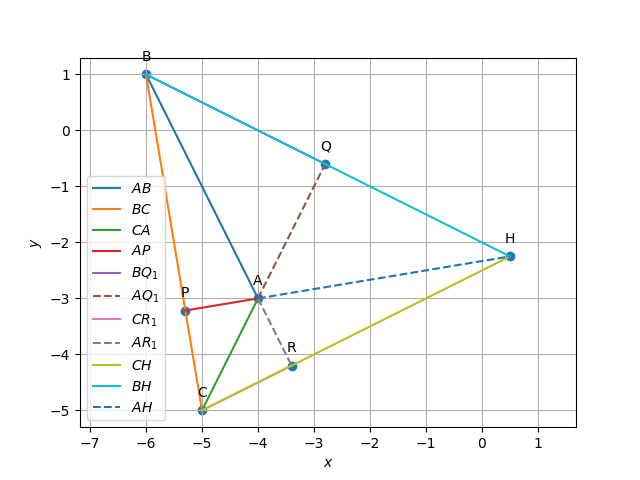
\includegraphics[width=0.8\linewidth] {/home/yogitha/triangle/figs/Fig3.png}
\caption{Altitudes}
\label{fig3}
\end{figure}
\begin{table}[!ht]
        \centering
        \caption{Perpendicular bisectors}
	\label{Table 4}	
	%%%%%%%%%%%%%%%%%%%%%%%%%%%%%%%%%%%%%%%%%%%%%%%%%%%%%%%%%%%%%%%%%%%%%%
%%                                                                  %%
%%  This is the header of a LaTeX2e file exported from Gnumeric.    %%
%%                                                                  %%
%%  This file can be compiled as it stands or included in another   %%
%%  LaTeX document. The table is based on the longtable package so  %%
%%  the longtable options (headers, footers...) can be set in the   %%
%%  preamble section below (see PRAMBLE).                           %%
%%                                                                  %%
%%  To include the file in another, the following two lines must be %%
%%  in the including file:                                          %%
%%        \def\inputGnumericTable{}                                 %%
%%  at the beginning of the file and:                               %%
%%        \input{name-of-this-file.tex}                             %%
%%  where the table is to be placed. Note also that the including   %%
%%  file must use the following packages for the table to be        %%
%%  rendered correctly:                                             %%
%%    \usepackage[latin1]{inputenc}                                 %%
%%    \usepackage{color}                                            %%
%%    \usepackage{array}                                            %%
%%    \usepackage{longtable}                                        %%
%%    \usepackage{calc}                                             %%
%%    \usepackage{multirow}                                         %%
%%    \usepackage{hhline}                                           %%
%%    \usepackage{ifthen}                                           %%
%%  optionally (for landscape tables embedded in another document): %%
%%    \usepackage{lscape}                                           %%
%%                                                                  %%
%%%%%%%%%%%%%%%%%%%%%%%%%%%%%%%%%%%%%%%%%%%%%%%%%%%%%%%%%%%%%%%%%%%%%%



%%  This section checks if we are begin input into another file or  %%
%%  the file will be compiled alone. First use a macro taken from   %%
%%  the TeXbook ex 7.7 (suggestion of Han-Wen Nienhuys).            %%
\def\ifundefined#1{\expandafter\ifx\csname#1\endcsname\relax}


%%  Check for the \def token for inputed files. If it is not        %%
%%  defined, the file will be processed as a standalone and the     %%
%%  preamble will be used.                                          %%
\ifundefined{inputGnumericTable}

%%  We must be able to close or not the document at the end.        %%
	\def\gnumericTableEnd{\end{document}}


%%%%%%%%%%%%%%%%%%%%%%%%%%%%%%%%%%%%%%%%%%%%%%%%%%%%%%%%%%%%%%%%%%%%%%
%%                                                                  %%
%%  This is the PREAMBLE. Change these values to get the right      %%
%%  paper size and other niceties.                                  %%
%%                                                                  %%
%%%%%%%%%%%%%%%%%%%%%%%%%%%%%%%%%%%%%%%%%%%%%%%%%%%%%%%%%%%%%%%%%%%%%%

	\documentclass[12pt%
			  %,landscape%
                    ]{report}
       \usepackage[latin1]{inputenc}
       \usepackage{fullpage}
       \usepackage{color}
       \usepackage{array}
       \usepackage{longtable}
       \usepackage{calc}
       \usepackage{multirow}
       \usepackage{hhline}
       \usepackage{ifthen}

	\begin{document}


%%  End of the preamble for the standalone. The next section is for %%
%%  documents which are included into other LaTeX2e files.          %%
\else

%%  We are not a stand alone document. For a regular table, we will %%
%%  have no preamble and only define the closing to mean nothing.   %%
    \def\gnumericTableEnd{}

%%  If we want landscape mode in an embedded document, comment out  %%
%%  the line above and uncomment the two below. The table will      %%
%%  begin on a new page and run in landscape mode.                  %%
%       \def\gnumericTableEnd{\end{landscape}}
%       \begin{landscape}


%%  End of the else clause for this file being \input.              %%
\fi

%%%%%%%%%%%%%%%%%%%%%%%%%%%%%%%%%%%%%%%%%%%%%%%%%%%%%%%%%%%%%%%%%%%%%%
%%                                                                  %%
%%  The rest is the gnumeric table, except for the closing          %%
%%  statement. Changes below will alter the table's appearance.     %%
%%                                                                  %%
%%%%%%%%%%%%%%%%%%%%%%%%%%%%%%%%%%%%%%%%%%%%%%%%%%%%%%%%%%%%%%%%%%%%%%

\providecommand{\gnumericmathit}[1]{#1} 
%%  Uncomment the next line if you would like your numbers to be in %%
%%  italics if they are italizised in the gnumeric table.           %%
%\renewcommand{\gnumericmathit}[1]{\mathit{#1}}
\providecommand{\gnumericPB}[1]%
{\let\gnumericTemp=\\#1\let\\=\gnumericTemp\hspace{0pt}}
 \ifundefined{gnumericTableWidthDefined}
        \newlength{\gnumericTableWidth}
        \newlength{\gnumericTableWidthComplete}
        \newlength{\gnumericMultiRowLength}
        \global\def\gnumericTableWidthDefined{}
 \fi
%% The following setting protects this code from babel shorthands.  %%
 \ifthenelse{\isundefined{\languageshorthands}}{}{\languageshorthands{english}}
%%  The default table format retains the relative column widths of  %%
%%  gnumeric. They can easily be changed to c, r or l. In that case %%
%%  you may want to comment out the next line and uncomment the one %%
%%  thereafter                                                      %%
\providecommand\gnumbox{\makebox[0pt]}
%%\providecommand\gnumbox[1][]{\makebox}

%% to adjust positions in multirow situations                       %%
\setlength{\bigstrutjot}{\jot}
\setlength{\extrarowheight}{\doublerulesep}

%%  The \setlongtables command keeps column widths the same across  %%
%%  pages. Simply comment out next line for varying column widths.  %%
\setlongtables

\setlength\gnumericTableWidth{%
	53pt+%
	53pt+%
	53pt+%
	53pt+%
	53pt+%
	53pt+%
	53pt+%
0pt}
\def\gumericNumCols{7}
\setlength\gnumericTableWidthComplete{\gnumericTableWidth+%
         \tabcolsep*\gumericNumCols*2+\arrayrulewidth*\gumericNumCols}
\ifthenelse{\lengthtest{\gnumericTableWidthComplete > \linewidth}}%
         {\def\gnumericScale{1*\ratio{\linewidth-%
                        \tabcolsep*\gumericNumCols*2-%
                        \arrayrulewidth*\gumericNumCols}%
{\gnumericTableWidth}}}%
{\def\gnumericScale{1}}

%%%%%%%%%%%%%%%%%%%%%%%%%%%%%%%%%%%%%%%%%%%%%%%%%%%%%%%%%%%%%%%%%%%%%%
%%                                                                  %%
%% The following are the widths of the various columns. We are      %%
%% defining them here because then they are easier to change.       %%
%% Depending on the cell formats we may use them more than once.    %%
%%                                                                  %%
%%%%%%%%%%%%%%%%%%%%%%%%%%%%%%%%%%%%%%%%%%%%%%%%%%%%%%%%%%%%%%%%%%%%%%

\ifthenelse{\isundefined{\gnumericColA}}{\newlength{\gnumericColA}}{}\settowidth{\gnumericColA}{\begin{tabular}{@{}p{53pt*\gnumericScale}@{}}x\end{tabular}}
\ifthenelse{\isundefined{\gnumericColB}}{\newlength{\gnumericColB}}{}\settowidth{\gnumericColB}{\begin{tabular}{@{}p{53pt*\gnumericScale}@{}}x\end{tabular}}
\ifthenelse{\isundefined{\gnumericColC}}{\newlength{\gnumericColC}}{}\settowidth{\gnumericColC}{\begin{tabular}{@{}p{53pt*\gnumericScale}@{}}x\end{tabular}}
\ifthenelse{\isundefined{\gnumericColD}}{\newlength{\gnumericColD}}{}\settowidth{\gnumericColD}{\begin{tabular}{@{}p{53pt*\gnumericScale}@{}}x\end{tabular}}
\ifthenelse{\isundefined{\gnumericColE}}{\newlength{\gnumericColE}}{}\settowidth{\gnumericColE}{\begin{tabular}{@{}p{53pt*\gnumericScale}@{}}x\end{tabular}}
\ifthenelse{\isundefined{\gnumericColF}}{\newlength{\gnumericColF}}{}\settowidth{\gnumericColF}{\begin{tabular}{@{}p{53pt*\gnumericScale}@{}}x\end{tabular}}
\ifthenelse{\isundefined{\gnumericColG}}{\newlength{\gnumericColG}}{}\settowidth{\gnumericColG}{\begin{tabular}{@{}p{53pt*\gnumericScale}@{}}x\end{tabular}}

\begin{tabular}[c]{%
	b{\gnumericColA}%
	b{\gnumericColB}%
	b{\gnumericColC}%
	b{\gnumericColD}%
	b{\gnumericColE}%
	b{\gnumericColF}%
	b{\gnumericColG}%
	}

%%%%%%%%%%%%%%%%%%%%%%%%%%%%%%%%%%%%%%%%%%%%%%%%%%%%%%%%%%%%%%%%%%%%%%
%%  The longtable options. (Caption, headers... see Goosens, p.124) %%
%	\caption{The Table Caption.}             \\	%
% \hline	% Across the top of the table.
%%  The rest of these options are table rows which are placed on    %%
%%  the first, last or every page. Use \multicolumn if you want.    %%

%%  Header for the first page.                                      %%
%	\multicolumn{7}{c}{The First Header} \\ \hline 
%	\multicolumn{1}{c}{colTag}	%Column 1
%	&\multicolumn{1}{c}{colTag}	%Column 2
%	&\multicolumn{1}{c}{colTag}	%Column 3
%	&\multicolumn{1}{c}{colTag}	%Column 4
%	&\multicolumn{1}{c}{colTag}	%Column 5
%	&\multicolumn{1}{c}{colTag}	%Column 6
%	&\multicolumn{1}{c}{colTag}	\\ \hline %Last column
%	\endfirsthead

%%  The running header definition.                                  %%
%	\hline
%	\multicolumn{7}{l}{\ldots\small\slshape continued} \\ \hline
%	\multicolumn{1}{c}{colTag}	%Column 1
%	&\multicolumn{1}{c}{colTag}	%Column 2
%	&\multicolumn{1}{c}{colTag}	%Column 3
%	&\multicolumn{1}{c}{colTag}	%Column 4
%	&\multicolumn{1}{c}{colTag}	%Column 5
%	&\multicolumn{1}{c}{colTag}	%Column 6
%	&\multicolumn{1}{c}{colTag}	\\ \hline %Last column
%	\endhead

%%  The running footer definition.                                  %%
%	\hline
%	\multicolumn{7}{r}{\small\slshape continued\ldots} \\
%	\endfoot

%%  The ending footer definition.                                   %%
%	\multicolumn{7}{c}{That's all folks} \\ \hline 
%	\endlastfoot
%%%%%%%%%%%%%%%%%%%%%%%%%%%%%%%%%%%%%%%%%%%%%%%%%%%%%%%%%%%%%%%%%%%%%%

\hhline{|--|--|---}
	 \multicolumn{2}{|p{	\gnumericColA+%
	\gnumericColB+%
	\tabcolsep*2*1}|}%
	{\gnumericPB{\centering}\gnumbox{parameters}}
	&\multicolumn{2}{p{	\gnumericColC+%
	\gnumericColD+%
	\tabcolsep*2*1}|}%
	{\gnumericPB{\centering}\gnumbox{value}}
	&\multicolumn{3}{p{	\gnumericColE+%
	\gnumericColF+%
	\gnumericColG+%
	\tabcolsep*2*2}|}%
	{\gnumericPB{\centering}\gnumbox{description}}
\\
\hhline{|-------|}
	 \multicolumn{2}{|p{	\gnumericColA+%
	\gnumericColB+%
	\tabcolsep*2*1}|}%
	{\gnumericPB{\centering}\gnumbox{$\vec{m_{10}}$}}
	&\multicolumn{2}{p{	\gnumericColC+%
	\gnumericColD+%
	\tabcolsep*2*1}|}%
	{\gnumericPB{\centering}\gnumbox{$\myvec{-6\\-1}$}}
	&\multicolumn{3}{c|}%
	{\setlength{\gnumericMultiRowLength}{0pt}%
	 \addtolength{\gnumericMultiRowLength}{\gnumericColE}%
	 \addtolength{\gnumericMultiRowLength}{\gnumericColF}%
	 \addtolength{\gnumericMultiRowLength}{\tabcolsep}%
	 \addtolength{\gnumericMultiRowLength}{\gnumericColG}%
	 \addtolength{\gnumericMultiRowLength}{\tabcolsep}%
	 \multirow{3}[1]{\gnumericMultiRowLength}{\parbox{\gnumericMultiRowLength}{%
	 \gnumericPB{\centering}\gnumbox{$AD_1$}}}}
\\
\hhline{|----|~~~}
	 \multicolumn{2}{|p{	\gnumericColA+%
	\gnumericColB+%
	\tabcolsep*2*1}|}%
	{\gnumericPB{\centering}\gnumbox{$\vec{n_{10}}$}}
	&\multicolumn{2}{p{	\gnumericColC+%
	\gnumericColD+%
	\tabcolsep*2*1}|}%
	{\gnumericPB{\centering}\gnumbox{$\myvec{1\\-6}$}}
	&
	&
	&\multicolumn{1}{p{\gnumericColG}|}%
	{}
\\
\hhline{|----|~~~}
	 \multicolumn{2}{|p{	\gnumericColA+%
	\gnumericColB+%
	\tabcolsep*2*1}|}%
	{\gnumericPB{\centering}\gnumbox{$c_{10}$}}
	&\multicolumn{2}{p{	\gnumericColC+%
	\gnumericColD+%
	\tabcolsep*2*1}|}%
	{\gnumericPB{\centering}\gnumbox{$\frac{13}{2}$}}
	&
	&
	&\multicolumn{1}{p{\gnumericColG}|}%
	{}
\\
\hhline{|-------|}
	 \multicolumn{2}{|p{	\gnumericColA+%
	\gnumericColB+%
	\tabcolsep*2*1}|}%
	{\gnumericPB{\centering}\gnumbox{$\vec{m_{11}}$}}
	&\multicolumn{2}{p{	\gnumericColC+%
	\gnumericColD+%
	\tabcolsep*2*1}|}%
	{\gnumericPB{\centering}\gnumbox{$\myvec{2\\1}$}}
	&\multicolumn{3}{c|}%
	{\setlength{\gnumericMultiRowLength}{0pt}%
	 \addtolength{\gnumericMultiRowLength}{\gnumericColE}%
	 \addtolength{\gnumericMultiRowLength}{\gnumericColF}%
	 \addtolength{\gnumericMultiRowLength}{\tabcolsep}%
	 \addtolength{\gnumericMultiRowLength}{\gnumericColG}%
	 \addtolength{\gnumericMultiRowLength}{\tabcolsep}%
	 \multirow{3}[1]{\gnumericMultiRowLength}{\parbox{\gnumericMultiRowLength}{%
	 \gnumericPB{\centering}\gnumbox{$BE_1$}}}}
\\
\hhline{|----|~~~}
	 \multicolumn{2}{|p{	\gnumericColA+%
	\gnumericColB+%
	\tabcolsep*2*1}|}%
	{\gnumericPB{\centering}\gnumbox{$\vec{n_{11}}$}}
	&\multicolumn{2}{p{	\gnumericColC+%
	\gnumericColD+%
	\tabcolsep*2*1}|}%
	{\gnumericPB{\centering}\gnumbox{$\myvec{-1\\2}$}}
	&
	&
	&\multicolumn{1}{p{\gnumericColG}|}%
	{}
\\
\hhline{|----|~~~}
	 \multicolumn{2}{|p{	\gnumericColA+%
	\gnumericColB+%
	\tabcolsep*2*1}|}%
	{\gnumericPB{\centering}\gnumbox{$c_{11}$}}
	&\multicolumn{2}{p{	\gnumericColC+%
	\gnumericColD+%
	\tabcolsep*2*1}|}%
	{\gnumericPB{\centering}\gnumbox{$\frac{-25}{2}$}}
	&
	&
	&\multicolumn{1}{p{\gnumericColG}|}%
	{}
\\
\hhline{|-------|}
	 \multicolumn{2}{|p{	\gnumericColA+%
	\gnumericColB+%
	\tabcolsep*2*1}|}%
	{\gnumericPB{\centering}\gnumbox{$\vec{m_{12}}$}}
	&\multicolumn{2}{p{	\gnumericColC+%
	\gnumericColD+%
	\tabcolsep*2*1}|}%
	{\gnumericPB{\centering}\gnumbox{$\myvec{4\\2}$}}
	&\multicolumn{3}{c|}%
	{\setlength{\gnumericMultiRowLength}{0pt}%
	 \addtolength{\gnumericMultiRowLength}{\gnumericColE}%
	 \addtolength{\gnumericMultiRowLength}{\gnumericColF}%
	 \addtolength{\gnumericMultiRowLength}{\tabcolsep}%
	 \addtolength{\gnumericMultiRowLength}{\gnumericColG}%
	 \addtolength{\gnumericMultiRowLength}{\tabcolsep}%
	 \multirow{3}[1]{\gnumericMultiRowLength}{\parbox{\gnumericMultiRowLength}{%
	 \gnumericPB{\centering}\gnumbox{$CF_1$}}}}
\\
\hhline{|----|~~~}
	 \multicolumn{2}{|p{	\gnumericColA+%
	\gnumericColB+%
	\tabcolsep*2*1}|}%
	{\gnumericPB{\centering}\gnumbox{$\vec{n_{12}}$}}
	&\multicolumn{2}{p{	\gnumericColC+%
	\gnumericColD+%
	\tabcolsep*2*1}|}%
	{\gnumericPB{\centering}\gnumbox{$\myvec{-2\\4}$}}
	&
	&
	&\multicolumn{1}{p{\gnumericColG}|}%
	{}
\\
\hhline{|----|~~~}
	 \multicolumn{2}{|p{	\gnumericColA+%
	\gnumericColB+%
	\tabcolsep*2*1}|}%
	{\gnumericPB{\centering}\gnumbox{$c_{12}$}}
	&\multicolumn{2}{p{	\gnumericColC+%
	\gnumericColD+%
	\tabcolsep*2*1}|}%
	{\gnumericPB{\centering}\gnumbox{6}}
	&
	&
	&\multicolumn{1}{p{\gnumericColG}|}%
	{}
\\
\hhline{|-------|}
	 \multicolumn{2}{|p{	\gnumericColA+%
	\gnumericColB+%
	\tabcolsep*2*1}|}%
	{\gnumericPB{\centering}\gnumbox{$\vec{O}$}}
	&\multicolumn{2}{p{	\gnumericColC+%
	\gnumericColD+%
	\tabcolsep*2*1}|}%
	{\gnumericPB{\centering}\gnumbox{$\myvec{\frac{31}{4}\\\frac{-119}{50}}$}}
	&\multicolumn{3}{p{	\gnumericColE+%
	\gnumericColF+%
	\gnumericColG+%
	\tabcolsep*2*2}|}%
	{\gnumericPB{\centering}\gnumbox{Circumcentre}}
\\
\hhline{|-------|}
	 \multicolumn{2}{|p{	\gnumericColA+%
	\gnumericColB+%
	\tabcolsep*2*1}|}%
	{\gnumericPB{\centering}\gnumbox{$\norm{\vec{O}-\vec{A}}$}}
	&\multicolumn{2}{c|}%
	{\setlength{\gnumericMultiRowLength}{0pt}%
	 \addtolength{\gnumericMultiRowLength}{\gnumericColC}%
	 \addtolength{\gnumericMultiRowLength}{\gnumericColD}%
	 \addtolength{\gnumericMultiRowLength}{\tabcolsep}%
	 \multirow{4}[2]{\gnumericMultiRowLength}{\parbox{\gnumericMultiRowLength}{%
	 \gnumericPB{\centering}\gnumbox{3.801}}}}
	&\multicolumn{3}{c|}%
	{\setlength{\gnumericMultiRowLength}{0pt}%
	 \addtolength{\gnumericMultiRowLength}{\gnumericColE}%
	 \addtolength{\gnumericMultiRowLength}{\gnumericColF}%
	 \addtolength{\gnumericMultiRowLength}{\tabcolsep}%
	 \addtolength{\gnumericMultiRowLength}{\gnumericColG}%
	 \addtolength{\gnumericMultiRowLength}{\tabcolsep}%
	 \multirow{4}[2]{\gnumericMultiRowLength}{\parbox{\gnumericMultiRowLength}{%
	 \gnumericPB{\centering}\gnumbox{$OA=OB=OC=R$}}}}
\\
\hhline{|--|~~~~~}
	 \multicolumn{2}{|p{	\gnumericColA+%
	\gnumericColB+%
	\tabcolsep*2*1}|}%
	{\gnumericPB{\centering}\gnumbox{$\norm{\vec{O}-\vec{B}}$}}
	&
	&\multicolumn{1}{p{\gnumericColD}|}%
	{}
	&
	&
	&\multicolumn{1}{p{\gnumericColG}|}%
	{}
\\
\hhline{|--|~~~~~}
	 \multicolumn{2}{|p{	\gnumericColA+%
	\gnumericColB+%
	\tabcolsep*2*1}|}%
	{\gnumericPB{\centering}\gnumbox{$\norm{\vec{O}-\vec{C}}$}}
	&
	&\multicolumn{1}{p{\gnumericColD}|}%
	{}
	&
	&
	&\multicolumn{1}{p{\gnumericColG}|}%
	{}
\\
\hhline{|--|~~~~~}
	 \multicolumn{2}{|p{	\gnumericColA+%
	\gnumericColB+%
	\tabcolsep*2*1}|}%
	{\gnumericPB{\centering}\gnumbox{$R$}}
	&
	&\multicolumn{1}{p{\gnumericColD}|}%
	{}
	&
	&
	&\multicolumn{1}{p{\gnumericColG}|}%
	{}
\\
\hhline{|-------|}
	 \multicolumn{2}{|p{	\gnumericColA+%
	\gnumericColB+%
	\tabcolsep*2*1}|}%
	{\gnumericPB{\centering}\gnumbox{$\angle BOC$}}
	&\multicolumn{2}{p{	\gnumericColC+%
	\gnumericColD+%
	\tabcolsep*2*1}|}%
	{\gnumericPB{\centering}\gnumbox{$253.73 \degree$}}
	&\multicolumn{3}{c|}%
	{\setlength{\gnumericMultiRowLength}{0pt}%
	 \addtolength{\gnumericMultiRowLength}{\gnumericColE}%
	 \addtolength{\gnumericMultiRowLength}{\gnumericColF}%
	 \addtolength{\gnumericMultiRowLength}{\tabcolsep}%
	 \addtolength{\gnumericMultiRowLength}{\gnumericColG}%
	 \addtolength{\gnumericMultiRowLength}{\tabcolsep}%
	 \multirow{2}[1]{\gnumericMultiRowLength}{\parbox{\gnumericMultiRowLength}{%
	 \gnumericPB{\centering}\gnumbox{$\angle BOC=2 \angle BAC$}}}}
\\
\hhline{|----|~~~}
	 \multicolumn{2}{|p{	\gnumericColA+%
	\gnumericColB+%
	\tabcolsep*2*1}|}%
	{\gnumericPB{\centering}\gnumbox{$\angle BAC$}}
	&\multicolumn{2}{p{	\gnumericColC+%
	\gnumericColD+%
	\tabcolsep*2*1}|}%
	{\gnumericPB{\centering}\gnumbox{$126.86 \degree$}}
	&
	&
	&\multicolumn{1}{p{\gnumericColG}|}%
	{}
\\

\hhline{|--|--|---|}
\end{tabular}

\ifthenelse{\isundefined{\languageshorthands}}{}{\languageshorthands{\languagename}}
\gnumericTableEnd

\end{table}
\begin{figure}[h!]
\centering
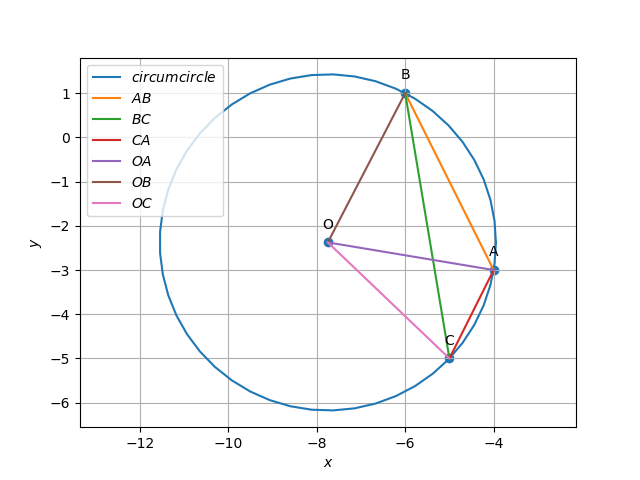
\includegraphics[width=0.8\linewidth] {/home/yogitha/triangle/figs/Fig4.png}
\caption{Perpendicular bisectors}
\label{fig4}
\end{figure}
\begin{table}[!ht]
        \centering
        \caption{Angular bisectors}
	\label{table 5}	
	%%%%%%%%%%%%%%%%%%%%%%%%%%%%%%%%%%%%%%%%%%%%%%%%%%%%%%%%%%%%%%%%%%%%%%
%%                                                                  %%
%%  This is the header of a LaTeX2e file exported from Gnumeric.    %%
%%                                                                  %%
%%  This file can be compiled as it stands or included in another   %%
%%  LaTeX document. The table is based on the longtable package so  %%
%%  the longtable options (headers, footers...) can be set in the   %%
%%  preamble section below (see PRAMBLE).                           %%
%%                                                                  %%
%%  To include the file in another, the following two lines must be %%
%%  in the including file:                                          %%
%%        \def\inputGnumericTable{}                                 %%
%%  at the beginning of the file and:                               %%
%%        \input{name-of-this-file.tex}                             %%
%%  where the table is to be placed. Note also that the including   %%
%%  file must use the following packages for the table to be        %%
%%  rendered correctly:                                             %%
%%    \usepackage[latin1]{inputenc}                                 %%
%%    \usepackage{color}                                            %%
%%    \usepackage{array}                                            %%
%%    \usepackage{longtable}                                        %%
%%    \usepackage{calc}                                             %%
%%    \usepackage{multirow}                                         %%
%%    \usepackage{hhline}                                           %%
%%    \usepackage{ifthen}                                           %%
%%  optionally (for landscape tables embedded in another document): %%
%%    \usepackage{lscape}                                           %%
%%                                                                  %%
%%%%%%%%%%%%%%%%%%%%%%%%%%%%%%%%%%%%%%%%%%%%%%%%%%%%%%%%%%%%%%%%%%%%%%



%%  This section checks if we are begin input into another file or  %%
%%  the file will be compiled alone. First use a macro taken from   %%
%%  the TeXbook ex 7.7 (suggestion of Han-Wen Nienhuys).            %%
\def\ifundefined#1{\expandafter\ifx\csname#1\endcsname\relax}


%%  Check for the \def token for inputed files. If it is not        %%
%%  defined, the file will be processed as a standalone and the     %%
%%  preamble will be used.                                          %%
\ifundefined{inputGnumericTable}

%%  We must be able to close or not the document at the end.        %%
	\def\gnumericTableEnd{\end{document}}


%%%%%%%%%%%%%%%%%%%%%%%%%%%%%%%%%%%%%%%%%%%%%%%%%%%%%%%%%%%%%%%%%%%%%%
%%                                                                  %%
%%  This is the PREAMBLE. Change these values to get the right      %%
%%  paper size and other niceties.                                  %%
%%                                                                  %%
%%%%%%%%%%%%%%%%%%%%%%%%%%%%%%%%%%%%%%%%%%%%%%%%%%%%%%%%%%%%%%%%%%%%%%

	\documentclass[12pt%
			  %,landscape%
                    ]{report}
       \usepackage[latin1]{inputenc}
       \usepackage{fullpage}
       \usepackage{color}
       \usepackage{array}
       \usepackage{longtable}
       \usepackage{calc}
       \usepackage{multirow}
       \usepackage{hhline}
       \usepackage{ifthen}

	\begin{document}


%%  End of the preamble for the standalone. The next section is for %%
%%  documents which are included into other LaTeX2e files.          %%
\else

%%  We are not a stand alone document. For a regular table, we will %%
%%  have no preamble and only define the closing to mean nothing.   %%
    \def\gnumericTableEnd{}

%%  If we want landscape mode in an embedded document, comment out  %%
%%  the line above and uncomment the two below. The table will      %%
%%  begin on a new page and run in landscape mode.                  %%
%       \def\gnumericTableEnd{\end{landscape}}
%       \begin{landscape}


%%  End of the else clause for this file being \input.              %%
\fi

%%%%%%%%%%%%%%%%%%%%%%%%%%%%%%%%%%%%%%%%%%%%%%%%%%%%%%%%%%%%%%%%%%%%%%
%%                                                                  %%
%%  The rest is the gnumeric table, except for the closing          %%
%%  statement. Changes below will alter the table's appearance.     %%
%%                                                                  %%
%%%%%%%%%%%%%%%%%%%%%%%%%%%%%%%%%%%%%%%%%%%%%%%%%%%%%%%%%%%%%%%%%%%%%%

\providecommand{\gnumericmathit}[1]{#1} 
%%  Uncomment the next line if you would like your numbers to be in %%
%%  italics if they are italizised in the gnumeric table.           %%
%\renewcommand{\gnumericmathit}[1]{\mathit{#1}}
\providecommand{\gnumericPB}[1]%
{\let\gnumericTemp=\\#1\let\\=\gnumericTemp\hspace{0pt}}
 \ifundefined{gnumericTableWidthDefined}
        \newlength{\gnumericTableWidth}
        \newlength{\gnumericTableWidthComplete}
        \newlength{\gnumericMultiRowLength}
        \global\def\gnumericTableWidthDefined{}
 \fi
%% The following setting protects this code from babel shorthands.  %%
 \ifthenelse{\isundefined{\languageshorthands}}{}{\languageshorthands{english}}
%%  The default table format retains the relative column widths of  %%
%%  gnumeric. They can easily be changed to c, r or l. In that case %%
%%  you may want to comment out the next line and uncomment the one %%
%%  thereafter                                                      %%
\providecommand\gnumbox{\makebox[0pt]}
%%\providecommand\gnumbox[1][]{\makebox}

%% to adjust positions in multirow situations                       %%
\setlength{\bigstrutjot}{\jot}
\setlength{\extrarowheight}{\doublerulesep}

%%  The \setlongtables command keeps column widths the same across  %%
%%  pages. Simply comment out next line for varying column widths.  %%
\setlongtables

\setlength\gnumericTableWidth{%
	53pt+%
	53pt+%
	53pt+%
	53pt+%
	53pt+%
	53pt+%
	53pt+%
0pt}
\def\gumericNumCols{7}
\setlength\gnumericTableWidthComplete{\gnumericTableWidth+%
         \tabcolsep*\gumericNumCols*2+\arrayrulewidth*\gumericNumCols}
\ifthenelse{\lengthtest{\gnumericTableWidthComplete > \linewidth}}%
         {\def\gnumericScale{1*\ratio{\linewidth-%
                        \tabcolsep*\gumericNumCols*2-%
                        \arrayrulewidth*\gumericNumCols}%
{\gnumericTableWidth}}}%
{\def\gnumericScale{1}}

%%%%%%%%%%%%%%%%%%%%%%%%%%%%%%%%%%%%%%%%%%%%%%%%%%%%%%%%%%%%%%%%%%%%%%
%%                                                                  %%
%% The following are the widths of the various columns. We are      %%
%% defining them here because then they are easier to change.       %%
%% Depending on the cell formats we may use them more than once.    %%
%%                                                                  %%
%%%%%%%%%%%%%%%%%%%%%%%%%%%%%%%%%%%%%%%%%%%%%%%%%%%%%%%%%%%%%%%%%%%%%%

\ifthenelse{\isundefined{\gnumericColA}}{\newlength{\gnumericColA}}{}\settowidth{\gnumericColA}{\begin{tabular}{@{}p{53pt*\gnumericScale}@{}}x\end{tabular}}
\ifthenelse{\isundefined{\gnumericColB}}{\newlength{\gnumericColB}}{}\settowidth{\gnumericColB}{\begin{tabular}{@{}p{53pt*\gnumericScale}@{}}x\end{tabular}}
\ifthenelse{\isundefined{\gnumericColC}}{\newlength{\gnumericColC}}{}\settowidth{\gnumericColC}{\begin{tabular}{@{}p{53pt*\gnumericScale}@{}}x\end{tabular}}
\ifthenelse{\isundefined{\gnumericColD}}{\newlength{\gnumericColD}}{}\settowidth{\gnumericColD}{\begin{tabular}{@{}p{53pt*\gnumericScale}@{}}x\end{tabular}}
\ifthenelse{\isundefined{\gnumericColE}}{\newlength{\gnumericColE}}{}\settowidth{\gnumericColE}{\begin{tabular}{@{}p{53pt*\gnumericScale}@{}}x\end{tabular}}
\ifthenelse{\isundefined{\gnumericColF}}{\newlength{\gnumericColF}}{}\settowidth{\gnumericColF}{\begin{tabular}{@{}p{53pt*\gnumericScale}@{}}x\end{tabular}}
\ifthenelse{\isundefined{\gnumericColG}}{\newlength{\gnumericColG}}{}\settowidth{\gnumericColG}{\begin{tabular}{@{}p{53pt*\gnumericScale}@{}}x\end{tabular}}

\begin{tabular}[c]{%
	b{\gnumericColA}%
	b{\gnumericColB}%
	b{\gnumericColC}%
	b{\gnumericColD}%
	b{\gnumericColE}%
	b{\gnumericColF}%
	b{\gnumericColG}%
	}

%%%%%%%%%%%%%%%%%%%%%%%%%%%%%%%%%%%%%%%%%%%%%%%%%%%%%%%%%%%%%%%%%%%%%%
%%  The longtable options. (Caption, headers... see Goosens, p.124) %%
%	\caption{The Table Caption.}             \\	%
% \hline	% Across the top of the table.
%%  The rest of these options are table rows which are placed on    %%
%%  the first, last or every page. Use \multicolumn if you want.    %%

%%  Header for the first page.                                      %%
%	\multicolumn{7}{c}{The First Header} \\ \hline 
%	\multicolumn{1}{c}{colTag}	%Column 1
%	&\multicolumn{1}{c}{colTag}	%Column 2
%	&\multicolumn{1}{c}{colTag}	%Column 3
%	&\multicolumn{1}{c}{colTag}	%Column 4
%	&\multicolumn{1}{c}{colTag}	%Column 5
%	&\multicolumn{1}{c}{colTag}	%Column 6
%	&\multicolumn{1}{c}{colTag}	\\ \hline %Last column
%	\endfirsthead

%%  The running header definition.                                  %%
%	\hline
%	\multicolumn{7}{l}{\ldots\small\slshape continued} \\ \hline
%	\multicolumn{1}{c}{colTag}	%Column 1
%	&\multicolumn{1}{c}{colTag}	%Column 2
%	&\multicolumn{1}{c}{colTag}	%Column 3
%	&\multicolumn{1}{c}{colTag}	%Column 4
%	&\multicolumn{1}{c}{colTag}	%Column 5
%	&\multicolumn{1}{c}{colTag}	%Column 6
%	&\multicolumn{1}{c}{colTag}	\\ \hline %Last column
%	\endhead

%%  The running footer definition.                                  %%
%	\hline
%	\multicolumn{7}{r}{\small\slshape continued\ldots} \\
%	\endfoot

%%  The ending footer definition.                                   %%
%	\multicolumn{7}{c}{That's all folks} \\ \hline 
%	\endlastfoot
%%%%%%%%%%%%%%%%%%%%%%%%%%%%%%%%%%%%%%%%%%%%%%%%%%%%%%%%%%%%%%%%%%%%%%

\hhline{|--|--|---}
	 \multicolumn{2}{|p{	\gnumericColA+%
	\gnumericColB+%
	\tabcolsep*2*1}|}%
	{\gnumericPB{\centering}\gnumbox{parameters}}
	&\multicolumn{2}{p{	\gnumericColC+%
	\gnumericColD+%
	\tabcolsep*2*1}|}%
	{\gnumericPB{\centering}\gnumbox{value}}
	&\multicolumn{3}{p{	\gnumericColE+%
	\gnumericColF+%
	\gnumericColG+%
	\tabcolsep*2*2}|}%
	{\gnumericPB{\centering}\gnumbox{description}}
\\
\hhline{|-------|}
	 \multicolumn{2}{|p{	\gnumericColA+%
	\gnumericColB+%
	\tabcolsep*2*1}|}%
	{\gnumericPB{\centering}\gnumbox{$\vec{m_{13}}$}}
	&\multicolumn{2}{p{	\gnumericColC+%
	\gnumericColD+%
	\tabcolsep*2*1}|}%
	{\gnumericPB{\centering}\gnumbox{$\myvec{0.89\\0}$}}
	&\multicolumn{3}{c|}%
	{\setlength{\gnumericMultiRowLength}{0pt}%
	 \addtolength{\gnumericMultiRowLength}{\gnumericColE}%
	 \addtolength{\gnumericMultiRowLength}{\gnumericColF}%
	 \addtolength{\gnumericMultiRowLength}{\tabcolsep}%
	 \addtolength{\gnumericMultiRowLength}{\gnumericColG}%
	 \addtolength{\gnumericMultiRowLength}{\tabcolsep}%
	 \multirow{3}[1]{\gnumericMultiRowLength}{\parbox{\gnumericMultiRowLength}{%
	 \gnumericPB{\centering}\gnumbox{$AI$}}}}
\\
\hhline{|----|~~~}
	 \multicolumn{2}{|p{	\gnumericColA+%
	\gnumericColB+%
	\tabcolsep*2*1}|}%
	{\gnumericPB{\centering}\gnumbox{$\vec{n_{13}}$}}
	&\multicolumn{2}{p{	\gnumericColC+%
	\gnumericColD+%
	\tabcolsep*2*1}|}%
	{\gnumericPB{\centering}\gnumbox{$\myvec{0\\0.89}$}}
	&
	&
	&\multicolumn{1}{p{\gnumericColG}|}%
	{}
\\
\hhline{|----|~~~}
	 \multicolumn{2}{|p{	\gnumericColA+%
	\gnumericColB+%
	\tabcolsep*2*1}|}%
	{\gnumericPB{\centering}\gnumbox{$c_{13}$}}
	&\multicolumn{2}{p{	\gnumericColC+%
	\gnumericColD+%
	\tabcolsep*2*1}|}%
	{\gnumericPB{\centering}\gnumbox{-2.68}}
	&
	&
	&\multicolumn{1}{p{\gnumericColG}|}%
	{}
\\
\hhline{|-------|}
	 \multicolumn{2}{|p{	\gnumericColA+%
	\gnumericColB+%
	\tabcolsep*2*1}|}%
	{\gnumericPB{\centering}\gnumbox{$\vec{m_{14}}$}}
	&\multicolumn{2}{p{	\gnumericColC+%
	\gnumericColD+%
	\tabcolsep*2*1}|}%
	{\gnumericPB{\centering}\gnumbox{$\myvec{-1.88\\-0.61}$}}
	&\multicolumn{3}{c|}%
	{\setlength{\gnumericMultiRowLength}{0pt}%
	 \addtolength{\gnumericMultiRowLength}{\gnumericColE}%
	 \addtolength{\gnumericMultiRowLength}{\gnumericColF}%
	 \addtolength{\gnumericMultiRowLength}{\tabcolsep}%
	 \addtolength{\gnumericMultiRowLength}{\gnumericColG}%
	 \addtolength{\gnumericMultiRowLength}{\tabcolsep}%
	 \multirow{3}[1]{\gnumericMultiRowLength}{\parbox{\gnumericMultiRowLength}{%
	 \gnumericPB{\centering}\gnumbox{$BI$}}}}
\\
\hhline{|----|~~~}
	 \multicolumn{2}{|p{	\gnumericColA+%
	\gnumericColB+%
	\tabcolsep*2*1}|}%
	{\gnumericPB{\centering}\gnumbox{$\vec{n_{14}}$}}
	&\multicolumn{2}{p{	\gnumericColC+%
	\gnumericColD+%
	\tabcolsep*2*1}|}%
	{\gnumericPB{\centering}\gnumbox{$\myvec{1.88\\-0.61}$}}
	&
	&
	&\multicolumn{1}{p{\gnumericColG}|}%
	{}
\\
\hhline{|----|~~~}
	 \multicolumn{2}{|p{	\gnumericColA+%
	\gnumericColB+%
	\tabcolsep*2*1}|}%
	{\gnumericPB{\centering}\gnumbox{$c_{14}$}}
	&\multicolumn{2}{p{	\gnumericColC+%
	\gnumericColD+%
	\tabcolsep*2*1}|}%
	{\gnumericPB{\centering}\gnumbox{10.67}}
	&
	&
	&\multicolumn{1}{p{\gnumericColG}|}%
	{}
\\
\hhline{|-------|}
	 \multicolumn{2}{|p{	\gnumericColA+%
	\gnumericColB+%
	\tabcolsep*2*1}|}%
	{\gnumericPB{\centering}\gnumbox{$\vec{m_{15}}$}}
	&\multicolumn{2}{p{	\gnumericColC+%
	\gnumericColD+%
	\tabcolsep*2*1}|}%
	{\gnumericPB{\centering}\gnumbox{$\myvec{-0.28\\-1.88}$}}
	&\multicolumn{3}{c|}%
	{\setlength{\gnumericMultiRowLength}{0pt}%
	 \addtolength{\gnumericMultiRowLength}{\gnumericColE}%
	 \addtolength{\gnumericMultiRowLength}{\gnumericColF}%
	 \addtolength{\gnumericMultiRowLength}{\tabcolsep}%
	 \addtolength{\gnumericMultiRowLength}{\gnumericColG}%
	 \addtolength{\gnumericMultiRowLength}{\tabcolsep}%
	 \multirow{3}[1]{\gnumericMultiRowLength}{\parbox{\gnumericMultiRowLength}{%
	 \gnumericPB{\centering}\gnumbox{$CI$}}}}
\\
\hhline{|----|~~~}
	 \multicolumn{2}{|p{	\gnumericColA+%
	\gnumericColB+%
	\tabcolsep*2*1}|}%
	{\gnumericPB{\centering}\gnumbox{$\vec{n_{15}}$}}
	&\multicolumn{2}{p{	\gnumericColC+%
	\gnumericColD+%
	\tabcolsep*2*1}|}%
	{\gnumericPB{\centering}\gnumbox{$\myvec{1.88\\-0.28}$}}
	&
	&
	&\multicolumn{1}{p{\gnumericColG}|}%
	{}
\\
\hhline{|----|~~~}
	 \multicolumn{2}{|p{	\gnumericColA+%
	\gnumericColB+%
	\tabcolsep*2*1}|}%
	{\gnumericPB{\centering}\gnumbox{$c_{15}$}}
	&\multicolumn{2}{p{	\gnumericColC+%
	\gnumericColD+%
	\tabcolsep*2*1}|}%
	{\gnumericPB{\centering}\gnumbox{-7.99}}
	&
	&
	&\multicolumn{1}{p{\gnumericColG}|}%
	{}
\\
\hhline{|-------|}
	 \multicolumn{2}{|p{	\gnumericColA+%
	\gnumericColB+%
	\tabcolsep*2*1}|}%
	{\gnumericPB{\centering}\gnumbox{$\vec{I}$}}
	&\multicolumn{2}{p{	\gnumericColC+%
	\gnumericColD+%
	\tabcolsep*2*1}|}%
	{\gnumericPB{\centering}\gnumbox{$\myvec{-4.7\\-3}$}}
	&\multicolumn{3}{p{	\gnumericColE+%
	\gnumericColF+%
	\gnumericColG+%
	\tabcolsep*2*2}|}%
	{\gnumericPB{\centering}\gnumbox{Incentre}}
\\
\hhline{|-------|}
	 \multicolumn{2}{|p{	\gnumericColA+%
	\gnumericColB+%
	\tabcolsep*2*1}|}%
	{\gnumericPB{\centering}\gnumbox{$\vec{D_3}$}}
	&\multicolumn{2}{p{	\gnumericColC+%
	\gnumericColD+%
	\tabcolsep*2*1}|}%
	{\gnumericPB{\centering}\gnumbox{$\myvec{-5.32\\-3.1}$}}
	&\multicolumn{3}{p{	\gnumericColE+%
	\gnumericColF+%
	\gnumericColG+%
	\tabcolsep*2*2}|}%
	{\gnumericPB{\centering}\gnumbox{Point of contact with $BC$}}
\\
\hhline{|-------|}
	 \multicolumn{2}{|p{	\gnumericColA+%
	\gnumericColB+%
	\tabcolsep*2*1}|}%
	{\gnumericPB{\centering}\gnumbox{$\vec{E_3}$}}
	&\multicolumn{2}{p{	\gnumericColC+%
	\gnumericColD+%
	\tabcolsep*2*1}|}%
	{\gnumericPB{\centering}\gnumbox{$\myvec{-4.14\\-3.28}$}}
	&\multicolumn{3}{p{	\gnumericColE+%
	\gnumericColF+%
	\gnumericColG+%
	\tabcolsep*2*2}|}%
	{\gnumericPB{\centering}\gnumbox{Point of contact with $AC$}}
\\
\hhline{|-------|}
	 \multicolumn{2}{|p{	\gnumericColA+%
	\gnumericColB+%
	\tabcolsep*2*1}|}%
	{\gnumericPB{\centering}\gnumbox{$\vec{F_3}$}}
	&\multicolumn{2}{p{	\gnumericColC+%
	\gnumericColD+%
	\tabcolsep*2*1}|}%
	{\gnumericPB{\centering}\gnumbox{$\myvec{-4.14\\-2.72}$}}
	&\multicolumn{3}{p{	\gnumericColE+%
	\gnumericColF+%
	\gnumericColG+%
	\tabcolsep*2*2}|}%
	{\gnumericPB{\centering}\gnumbox{Point of contact with $AB$}}
\\
\hhline{|-------|}
	 \multicolumn{2}{|p{	\gnumericColA+%
	\gnumericColB+%
	\tabcolsep*2*1}|}%
	{\gnumericPB{\centering}\gnumbox{$\norm{\vec{I}-\vec{D_3}}$}}
	&\multicolumn{2}{c|}%
	{\setlength{\gnumericMultiRowLength}{0pt}%
	 \addtolength{\gnumericMultiRowLength}{\gnumericColC}%
	 \addtolength{\gnumericMultiRowLength}{\gnumericColD}%
	 \addtolength{\gnumericMultiRowLength}{\tabcolsep}%
	 \multirow{4}[2]{\gnumericMultiRowLength}{\parbox{\gnumericMultiRowLength}{%
	 \gnumericPB{\centering}\gnumbox{0.625}}}}
	&\multicolumn{3}{c|}%
	{\setlength{\gnumericMultiRowLength}{0pt}%
	 \addtolength{\gnumericMultiRowLength}{\gnumericColE}%
	 \addtolength{\gnumericMultiRowLength}{\gnumericColF}%
	 \addtolength{\gnumericMultiRowLength}{\tabcolsep}%
	 \addtolength{\gnumericMultiRowLength}{\gnumericColG}%
	 \addtolength{\gnumericMultiRowLength}{\tabcolsep}%
	 \multirow{4}[2]{\gnumericMultiRowLength}{\parbox{\gnumericMultiRowLength}{%
	 \gnumericPB{\centering}\gnumbox{$ID_3=IE_3=IF_3=r$}}}}
\\
\hhline{|--|~~~~~}
	 \multicolumn{2}{|p{	\gnumericColA+%
	\gnumericColB+%
	\tabcolsep*2*1}|}%
	{\gnumericPB{\centering}\gnumbox{$\norm{\vec{I}-\vec{E_3}}$}}
	&
	&\multicolumn{1}{p{\gnumericColD}|}%
	{}
	&
	&
	&\multicolumn{1}{p{\gnumericColG}|}%
	{}
\\
\hhline{|--|~~~~~}
	 \multicolumn{2}{|p{	\gnumericColA+%
	\gnumericColB+%
	\tabcolsep*2*1}|}%
	{\gnumericPB{\centering}\gnumbox{$\norm{\vec{I}-\vec{F_3}}$}}
	&
	&\multicolumn{1}{p{\gnumericColD}|}%
	{}
	&
	&
	&\multicolumn{1}{p{\gnumericColG}|}%
	{}
\\
\hhline{|--|~~~~~}
	 \multicolumn{2}{|p{	\gnumericColA+%
	\gnumericColB+%
	\tabcolsep*2*1}|}%
	{\gnumericPB{\centering}\gnumbox{$r$}}
	&
	&\multicolumn{1}{p{\gnumericColD}|}%
	{}
	&
	&
	&\multicolumn{1}{p{\gnumericColG}|}%
	{}
\\
\hhline{|-------|}
	 \multicolumn{2}{|p{	\gnumericColA+%
	\gnumericColB+%
	\tabcolsep*2*1}|}%
	{\gnumericPB{\centering}\gnumbox{$\angle BAI$}}
	&\multicolumn{2}{c|}%
	{\setlength{\gnumericMultiRowLength}{0pt}%
	 \addtolength{\gnumericMultiRowLength}{\gnumericColC}%
	 \addtolength{\gnumericMultiRowLength}{\gnumericColD}%
	 \addtolength{\gnumericMultiRowLength}{\tabcolsep}%
	 \multirow{2}[1]{\gnumericMultiRowLength}{\parbox{\gnumericMultiRowLength}{%
	 \gnumericPB{\centering}\gnumbox{$13.28\degree$}}}}
	&\multicolumn{3}{c|}%
	{\setlength{\gnumericMultiRowLength}{0pt}%
	 \addtolength{\gnumericMultiRowLength}{\gnumericColE}%
	 \addtolength{\gnumericMultiRowLength}{\gnumericColF}%
	 \addtolength{\gnumericMultiRowLength}{\tabcolsep}%
	 \addtolength{\gnumericMultiRowLength}{\gnumericColG}%
	 \addtolength{\gnumericMultiRowLength}{\tabcolsep}%
	 \multirow{2}[1]{\gnumericMultiRowLength}{\parbox{\gnumericMultiRowLength}{%
	 \gnumericPB{\centering}\gnumbox{$\angle BAI=\angle CAI$}}}}
\\
\hhline{|--|~~~~~}
	 \multicolumn{2}{|p{	\gnumericColA+%
	\gnumericColB+%
	\tabcolsep*2*1}|}%
	{\gnumericPB{\centering}\gnumbox{$\angle CAI$}}
	&
	&\multicolumn{1}{p{\gnumericColD}|}%
	{}
	&
	&
	&\multicolumn{1}{p{\gnumericColG}|}%
	{}
\\
\hhline{|-------|}
	 \multicolumn{2}{|p{	\gnumericColA+%
	\gnumericColB+%
	\tabcolsep*2*1}|}%
	{\gnumericPB{\centering}\gnumbox{$\angle ABI$}}
	&\multicolumn{2}{c|}%
	{\setlength{\gnumericMultiRowLength}{0pt}%
	 \addtolength{\gnumericMultiRowLength}{\gnumericColC}%
	 \addtolength{\gnumericMultiRowLength}{\gnumericColD}%
	 \addtolength{\gnumericMultiRowLength}{\tabcolsep}%
	 \multirow{2}[1]{\gnumericMultiRowLength}{\parbox{\gnumericMultiRowLength}{%
	 \gnumericPB{\centering}\gnumbox{$9.21\degree$}}}}
	&\multicolumn{3}{c|}%
	{\setlength{\gnumericMultiRowLength}{0pt}%
	 \addtolength{\gnumericMultiRowLength}{\gnumericColE}%
	 \addtolength{\gnumericMultiRowLength}{\gnumericColF}%
	 \addtolength{\gnumericMultiRowLength}{\tabcolsep}%
	 \addtolength{\gnumericMultiRowLength}{\gnumericColG}%
	 \addtolength{\gnumericMultiRowLength}{\tabcolsep}%
	 \multirow{2}[1]{\gnumericMultiRowLength}{\parbox{\gnumericMultiRowLength}{%
	 \gnumericPB{\centering}\gnumbox{$\angle ABI=\angle CBI$}}}}
\\
\hhline{|--|~~~~~}
	 \multicolumn{2}{|p{	\gnumericColA+%
	\gnumericColB+%
	\tabcolsep*2*1}|}%
	{\gnumericPB{\centering}\gnumbox{$\angle CBI$}}
	&
	&\multicolumn{1}{p{\gnumericColD}|}%
	{}
	&
	&
	&\multicolumn{1}{p{\gnumericColG}|}%
	{}
\\
\hhline{|-------|}
	 \multicolumn{2}{|p{	\gnumericColA+%
	\gnumericColB+%
	\tabcolsep*2*1}|}%
	{\gnumericPB{\centering}\gnumbox{$\angle ACI$}}
	&\multicolumn{2}{c|}%
	{\setlength{\gnumericMultiRowLength}{0pt}%
	 \addtolength{\gnumericMultiRowLength}{\gnumericColC}%
	 \addtolength{\gnumericMultiRowLength}{\gnumericColD}%
	 \addtolength{\gnumericMultiRowLength}{\tabcolsep}%
	 \multirow{2}[1]{\gnumericMultiRowLength}{\parbox{\gnumericMultiRowLength}{%
	 \gnumericPB{\centering}\gnumbox{$67.5\degree$}}}}
	&\multicolumn{3}{c|}%
	{\setlength{\gnumericMultiRowLength}{0pt}%
	 \addtolength{\gnumericMultiRowLength}{\gnumericColE}%
	 \addtolength{\gnumericMultiRowLength}{\gnumericColF}%
	 \addtolength{\gnumericMultiRowLength}{\tabcolsep}%
	 \addtolength{\gnumericMultiRowLength}{\gnumericColG}%
	 \addtolength{\gnumericMultiRowLength}{\tabcolsep}%
	 \multirow{2}[1]{\gnumericMultiRowLength}{\parbox{\gnumericMultiRowLength}{%
	 \gnumericPB{\centering}\gnumbox{$\angle ACI=\angle BCI$}}}}
\\
\hhline{|--|~~~~~}
	 \multicolumn{2}{|p{	\gnumericColA+%
	\gnumericColB+%
	\tabcolsep*2*1}|}%
	{\gnumericPB{\centering}\gnumbox{$\angle BCI$}}
	&
	&\multicolumn{1}{p{\gnumericColD}|}%
	{}
	&
	&
	&\multicolumn{1}{p{\gnumericColG}|}%
	{}
\\
\hhline{|--|--|---|}
\end{tabular}

\ifthenelse{\isundefined{\languageshorthands}}{}{\languageshorthands{\languagename}}
\gnumericTableEnd

\end{table}
\begin{figure}[h!]
\centering
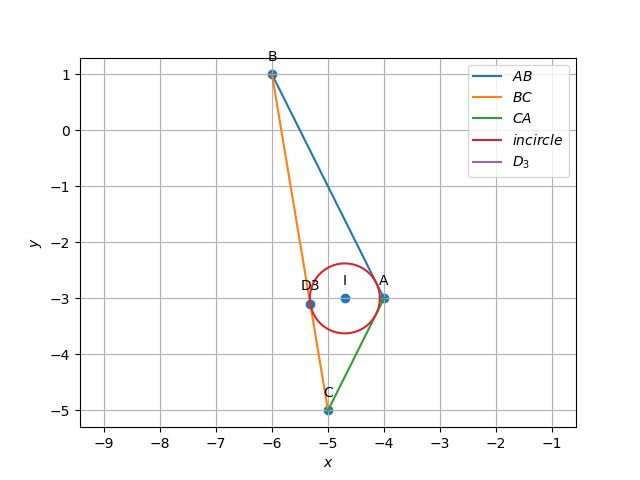
\includegraphics[width=0.8\linewidth] {/home/yogitha/triangle/figs/Fig5.png}
\caption{Angular bisectors}
\label{fig5}
\end{figure}
\end{document}
